\documentclass[type=bachelor]{thuthesis}
% 选项:
%   type=[bachelor|master|doctor|postdoctor], % 必选
%   secret,                                   % 可选
%   pifootnote,                               % 可选(建议打开)
%   openany|openright,                        % 可选,基本不用
%   arial,                                    % 可选,基本不用
%   arialtoc,                                 % 可选,基本不用
%   arialtitle                                % 可选,基本不用

% 所有其它可能用到的包都统一放到这里了,可以根据自己的实际添加或者删除。
\usepackage{thuthesis}

%%%%%%%%%
\usepackage{geometry}
\usepackage{tocbibind}
\usepackage{graphicx}%,floatrow}
\usepackage{amsmath}
\usepackage{amsfonts}
\usepackage{amssymb}
\usepackage{multirow}
% \usepackage{subfigure}
\usepackage{bm}
\usepackage{braket}
%\usepackage{staves} %package for peculiar symbols
\newcommand{\beqt}{ \begin{equation} }
\newcommand{\eeqt}{\end{equation}}
% \newcommand{\toprule}{\hline}
% \newcommand{\midrule}{\hline\hline}
% \newcommand{\bottomrule}{\hline}
\usepackage[framed,numbered,autolinebreaks,useliterate]{mcode}
%%%%%%%%%
% \usepackage{ctex}

% 定义所有的图片文件在 figures 子目录下
\graphicspath{{figures/}}

% 可以在这里修改配置文件中的定义。导言区可以使用中文。
% \def\myname{薛瑞尼}

\begin{document}


%%% 封面部分
\frontmatter
\thusetup{
  %******************************
  % 注意:
  %   1. 配置里面不要出现空行
  %   2. 不需要的配置信息可以删除
  %******************************
  %
  %=====
  % 秘级
  %=====
  secretlevel={秘密},
  secretyear={10},
  %
  %=========
  % 中文信息
  %=========
  % ctitle={清华大学学位论文 \LaTeX\ 模板\\使用示例文档 v\version},
  ctitle={基于超导量子比特与固态自旋的混合量子系统},
  cdegree={理学学士},
  cdepartment={物理系},
  cmajor={物理学},
  cauthor={蒋文韬},
  csupervisor={宋祎璞副研究员},
  % cassosupervisor={陈文光教授}, % 副指导老师
  % ccosupervisor={某某某教授}, % 联合指导老师
  % 日期自动使用当前时间,若需指定按如下方式修改:
  % cdate={超新星纪元},
  %
  % 博士后专有部分
  cfirstdiscipline={计算机科学与技术},
  cseconddiscipline={系统结构},
  postdoctordate={2009年7月——2011年7月},
  id={编号}, % 可以留空: id={},
  udc={UDC}, % 可以留空
  catalognumber={分类号}, % 可以留空
  %
  %=========
  % 英文信息
  %=========
  etitle={An Introduction to \LaTeX{} Thesis Template of Tsinghua University v\version},
  % 这块比较复杂,需要分情况讨论:
  % 1. 学术型硕士
  %    edegree:必须为Master of Arts或Master of Science(注意大小写)
  %             “哲学、文学、历史学、法学、教育学、艺术学门类,公共管理学科
  %              填写Master of Arts,其它填写Master of Science”
  %    emajor:“获得一级学科授权的学科填写一级学科名称,其它填写二级学科名称”
  % 2. 专业型硕士
  %    edegree:“填写专业学位英文名称全称”
  %    emajor:“工程硕士填写工程领域,其它专业学位不填写此项”
  % 3. 学术型博士
  %    edegree:Doctor of Philosophy(注意大小写)
  %    emajor:“获得一级学科授权的学科填写一级学科名称,其它填写二级学科名称”
  % 4. 专业型博士
  %    edegree:“填写专业学位英文名称全称”
  %    emajor:不填写此项
  edegree={Doctor of Engineering},
  emajor={Computer Science and Technology},
  eauthor={Xue Ruini},
  esupervisor={Professor Zheng Weimin},
  eassosupervisor={Chen Wenguang},
  % 日期自动生成,若需指定按如下方式修改:
  % edate={December, 2005}
  %
  % 关键词用“英文逗号”分割
  ckeywords={\TeX, \LaTeX, CJK, 模板, 论文},
  ekeywords={\TeX, \LaTeX, CJK, template, thesis}
}

% 定义中英文摘要和关键字
\begin{cabstract}
  论文的摘要是对论文研究内容和成果的高度概括。摘要应对论文所研究的问题及其研究目
  的进行描述,对研究方法和过程进行简单介绍,对研究成果和所得结论进行概括。摘要应
  具有独立性和自明性,其内容应包含与论文全文同等量的主要信息。使读者即使不阅读全
  文,通过摘要就能了解论文的总体内容和主要成果。

  论文摘要的书写应力求精确、简明。切忌写成对论文书写内容进行提要的形式,尤其要避
  免“第 1 章……;第 2 章……;……”这种或类似的陈述方式。

  本文介绍清华大学论文模板 \thuthesis{} 的使用方法。本模板符合学校的本科、硕士、
  博士论文格式要求。

  本文的创新点主要有:
  \begin{itemize}
    \item 用例子来解释模板的使用方法;
    \item 用废话来填充无关紧要的部分;
    \item 一边学习摸索一边编写新代码。
  \end{itemize}

  关键词是为了文献标引工作、用以表示全文主要内容信息的单词或术语。关键词不超过 5
  个,每个关键词中间用分号分隔。(模板作者注:关键词分隔符不用考虑,模板会自动处
  理。英文关键词同理。)
\end{cabstract}

% 如果习惯关键字跟在摘要文字后面,可以用直接命令来设置,如下:
% \ckeywords{\TeX, \LaTeX, CJK, 模板, 论文}

\begin{eabstract}
   An abstract of a dissertation is a summary and extraction of research work
   and contributions. Included in an abstract should be description of research
   topic and research objective, brief introduction to methodology and research
   process, and summarization of conclusion and contributions of the
   research. An abstract should be characterized by independence and clarity and
   carry identical information with the dissertation. It should be such that the
   general idea and major contributions of the dissertation are conveyed without
   reading the dissertation.

   An abstract should be concise and to the point. It is a misunderstanding to
   make an abstract an outline of the dissertation and words ``the first
   chapter'', ``the second chapter'' and the like should be avoided in the
   abstract.

   Key words are terms used in a dissertation for indexing, reflecting core
   information of the dissertation. An abstract may contain a maximum of 5 key
   words, with semi-colons used in between to separate one another.
\end{eabstract}

% \ekeywords{\TeX, \LaTeX, CJK, template, thesis}

% 如果使用授权说明扫描页,将可选参数中指定为扫描得到的 PDF 文件名,例如:
% \makecover[scan-auth.pdf]
\makecover

%% 目录
\tableofcontents

%% 符号对照表
\begin{denotation}[3cm]
\item[HPC] 高性能计算 (High Performance Computing)
\item[cluster] 集群
\item[Itanium] 安腾
\item[SMP] 对称多处理
\item[API] 应用程序编程接口
\item[PI] 聚酰亚胺
\item[MPI] 聚酰亚胺模型化合物,N-苯基邻苯酰亚胺
\item[PBI] 聚苯并咪唑
\item[MPBI] 聚苯并咪唑模型化合物,N-苯基苯并咪唑
\item[PY] 聚吡咙
\item[PMDA-BDA]	均苯四酸二酐与联苯四胺合成的聚吡咙薄膜
\item[$\Delta G$] 活化自由能 (Activation Free Energy)
\item[$\chi$] 传输系数 (Transmission Coefficient)
\item[$E$] 能量
\item[$m$] 质量
\item[$c$] 光速
\item[$P$] 概率
\item[$T$] 时间
\item[$v$] 速度
\item[劝学] 君子曰:学不可以已。青,取之于蓝,而青于蓝;冰,水为之,而寒于水。木
  直中绳。輮以为轮,其曲中规。虽有槁暴,不复挺者,輮使之然也。故木受绳则直,金就
  砺则利,君子博学而日参省乎己,则知明而行无过矣。吾尝终日而思矣,不如须臾之所学
  也;吾尝跂而望矣,不如登高之博见也。登高而招,臂非加长也,而见者远;顺风而呼,
  声非加疾也,而闻者彰。假舆马者,非利足也,而致千里;假舟楫者,非能水也,而绝江
  河,君子生非异也,善假于物也。积土成山,风雨兴焉;积水成渊,蛟龙生焉;积善成德,
  而神明自得,圣心备焉。故不积跬步,无以至千里;不积小流,无以成江海。骐骥一跃,
  不能十步;驽马十驾,功在不舍。锲而舍之,朽木不折;锲而不舍,金石可镂。蚓无爪牙
  之利,筋骨之强,上食埃土,下饮黄泉,用心一也。蟹六跪而二螯,非蛇鳝之穴无可寄托
  者,用心躁也。—— 荀况
\end{denotation}



%%% 正文部分
\mainmatter
%!TEX root = ../main.tex
\chapter{引言:基于超导量子比特与固态自旋的混合量子系统简介}
\label{cha:intro}




        自从量子理论于上世纪初被提出、建立与发展以来,对世界产生了众多深远的影响。而在1970到1980年间,一些学者开始以可设计的角度来看待与研究量子系统\cite{feynman1982simulating},这带来了一系列观念的变化,人们开始思考如何制备与设计量子系统,并且综合物理、计算机科学以及信息论来提出一些全新的问题。\cite{nielsen2002quantum}自从量子加密通信的BB84协议\cite{bennett1984quantum},量子搜索算法\cite{grover1996fast}与量子质因数分解算法\cite{shor1994algorithms}被提出后,人们看见了基于量子力学原理的计算机与通信系统能够在一些问题上达到超越经典系统的性能,进而促进了量子信息实验的进展。

        \section{混合量子系统的重要性与现有研究状况} % (fold)
        \label{sec:importance}

            基于量子力学的计算机的最基本的组成元素为量子比特。一个量子比特是一个二能级量子系统的统称。,为了满足组建量子计算机的目的,一个好的二能级系统需要可扩展,可初始化,退相干时间远大于单次操作时间,可构建任意的量子逻辑门,可被独立测量这五个条件\cite{divincenzo2000physical}。人们对许多不同的微观二能级系统进行了尝试,包括量子点\cite{loss1998quantum},离子阱\cite{haffner2008quantum},固态自旋系统\cite{gershenfeld1997bulk},超导量子比特\cite{devoret2013superconducting}以及线性光学\cite{kok2007linear}等。

            这些不同系统各自建立的量子比特有不同的特点,例如基于离子阱的量子比特有很高的操作与测量成功率,但其扩展性相对较差;超导量子比特有较好的扩展性,并且容易操作,但其退相干时间则相对较短;基于光子的量子比特则是量子通讯的最佳选择。因此,通过将不同量子系统耦合起来,分别利用他们各自的优点进行相应的操作,是量子计算与量子通信的发展趋势。本文主要关注由超导量子比特与固态自旋系统构成的混合量子系统。


            通过将量子比特的状态从相干时间较短但操作方便的系统转换到相干时间相对更长的系统,即可在量子计算与量子信息的存储两方面均达到较好的效果。利用自旋系综作为量子存储器的想法在近十年前便开始有人提出\cite{Dutt2007,Imamoglu2009,Wesenberg2009},并且进行了相关基础实验,如自旋系综与超导微波谐振腔的耦合\cite{Schuster2010},并且能够达到强耦合的程度\cite{kubo2010},也即耦合强度超过了自旋系综以及谐振腔的衰减与退相干速率。这些实验充分说明利用自旋系综与超导谐振腔耦合这一课题的重要性与意义。另一方面,也有直接将自旋系综或是单个自旋与超导量子比特进行耦合的相关理论计算\cite{Marcos2010}与实验工作\cite{Zhu2011,Mark2013}。这篇文章主要考虑单个自旋或自旋系综与谐振腔的耦合,进而通过谐振腔再与超导量子比特进行耦合,不考虑单个自旋或自旋系综与超导量子比特的直接耦合。通过自旋与谐振腔的耦合,还可以通过谐振腔达到量子极限的测量精度\cite{Bienfait2016a}以及通过谐振腔的Purcell效应控制自旋系综的能量衰减速率\cite{Bienfait2016b},这些都是十分有意义的工作。

            由于自旋通过谐振腔中的磁场与谐振腔形成耦合,磁场的不均匀性将导致自旋与谐振腔耦合强度的不均匀性。在提高谐振腔的磁场均匀性这个方面,有相关工作通过在传输线谐振腔的基础上增加中心传输线的条数达到改善谐振腔磁场均匀性的效果\cite{Benningshof2013,Mohebbi2014},也有相关工作从改良三维谐振腔的角度出发,在保持谐振腔中磁场的均匀性的效果前提下增加磁场强度进而增加耦合强度\cite{Angerer2016}。在单个自旋与谐振腔耦合这方面,通过改进电感部分的设计,可以局域地增强磁场强度,进而增大谐振腔与单个自旋的耦合强度\cite{Jenkins2014,Eichler2017},从而可能通过单个自旋达到强耦合的程度\cite{sarabi2017prospective}。

            本文将计算并重现对传输线谐振腔磁场的仿真计算并估计自旋与传输线谐振腔的耦合强度,也从改良三维谐振腔的角度进行了仿真。另一方面,本文仿真并改进了通过重新设计谐振腔电感部分以增强耦合强度的设计,并进一步开始尝试该设计的微纳加工实现,并整理了微纳加工流程。对制备出来的器件,通过PPMS测量系统进行了测量。本文的第\ref{cha:spin_simulation}章中介绍了前文提到的多个仿真工作。对于测量系统的搭建与改进的相关内容在第\ref{cha:PPMS测量系统}章中有详细介绍,并在第\ref{cha:2_5维谐振腔的制备与测量}章中展示了改良的谐振腔的微纳加工工艺并利用搭建的测量系统对其进行了测量。在附录\ref{cha:SCQubitPrinciple}中介绍了超导量子比特的基础知识,随后在附录\ref{cha:fabrication}中包含了微纳加工各个步骤的详细流程与相关参数。测量系统搭建过程中编写的控制程序也附于附录\ref{cha:measurement_code}中供查阅。




        \section{超导量子系统与常见固态自旋系统} % (fold)
        \label{sec:qubit_and_spin}

            常见的超导量子比特由以下哈密顿量描述:
            \begin{equation}
                H_{sc} = 4 E_C (\hat n - n_g)^2 -E_J \cos \hat \phi
            \end{equation}
            其中$ E_C $与$E_J$分别为电容能量与约瑟夫森能量,两者比值的不同取值范围对应不同的超导量子比特种类,本文的工作将集中关注Transmon超导量子比特,这种量子比特对应$E_J/E_C\sim 50$的量级\cite{koch2007charge}。通过哈密顿量可以看出,超导量子比特对应非线性的谐振子,其能级非均匀分布,因而可以控制其量子态处于两个选定的本征态构成的态空间内,一般选择其基态与第一激发态,进而近似作为一个两能级系统构成量子比特。经过一系列化简,可将Transmon超导量子比特的哈密顿量写成两能级系统的标准形式
            \begin{equation}
                H_{trans} = \frac{1}{2}\hbar \omega_a \sigma_z 
            \end{equation}
            其中$ \omega_a = \sqrt{8E_JE_C}/\hbar $为基态与第一激发态的能量差对应的频率。通过将超导量子比特与平面谐振腔进行耦合,即可进行超导量子比特的操作与读取。

            自旋为很多微观粒子具有的量子特性,如电子自旋与核自旋。因为自旋与环境作用相对较弱,因此具有较长的退相干时间,是理想的存储介质。常见的自旋系统如金刚石色心(NV centers),由金刚石中一个碳原子被氮原子替代,以及相邻的一个碳原子空缺共同组成,构成一个等效的自旋为一的量子系统,如图\ref{fig:NV_centers}所示。

            \begin{figure}[h]
                \centering
                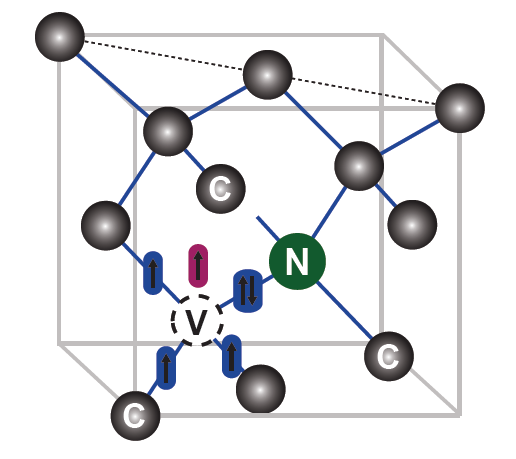
\includegraphics[width=3in]{NV.png}
                \caption{金刚石色心结构示意图,其中碳空位由V表示,氮掺杂由N表示\cite{grezes2016towards}。}
                \label{fig:NV_centers}
            \end{figure}%

            \begin{figure}[h]
                \centering
                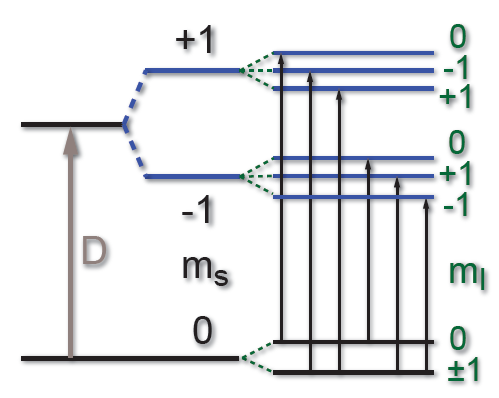
\includegraphics[width=3in]{NV_levels.png}
                \caption{金刚石色心在考虑零场劈裂与外加磁场后的能级示意图。其中$D$为零场劈裂导致的能级分裂,$m_S = \pm1$的两个态之间的能量差来源于应力与局域电场。不同核自旋量子数$m_I$的态之间的能级分裂来源于超精细相互作用\cite{grezes2016towards}。}
                \label{fig:NV_levels}
            \end{figure}

            考虑应力产生的零场劈裂以及外加静磁场后,一个金刚石色心中的自旋的简并能级发生分裂,相应的哈密顿量为\cite{grezes2016towards}
            \begin{equation}
            \label{eqn:NV_hamiltonian}
                H/\hbar = \bm S \cdot \bar{\bm D} \cdot \bm S - \gamma_e \bm B_{NV} \cdot \bm S + S \cdot \bar{\bm A}\cdot I +P I_Z^2
            \end{equation}
            其中$ \gamma_e = -g_e \mu_B /\hbar = -2\pi \times 2.8 \mathrm{MHz/Gs} $为NV电子自旋的旋磁比。$\bar{\bm D} $为零场劈裂张量,$\bm B_{NV} $为金刚石色心所处位置的磁场,$\bar{\bm A}$为超精细相互作用张量,最后一项为氮原子四极矩产生的能量项。知道了系统的哈密顿量后,即可选取两个态构成量子比特,这样近似下的哈密顿量与二能级系统的哈密顿量相同。通过将自旋与不同量子系统进行耦合,即可达到存储与读取量子信息的目的。
            




            

        \section{超导量子系统与自旋系综的耦合} % (fold)
        \label{sec:simulation_experimental_works}

            目前已有许多关于超导量子比特与固态自旋耦合的相关实验。由于自旋通过磁场与外界耦合,强度很弱,因此常采用自旋系综与平面波导谐振腔的磁场耦合,谐振腔再与超导量子比特耦合的方法\cite{grezes2016towards}。这种方法能够实现多次的存储与读取,本节将对这方面的理论工作与实验实现进行总结。

            首先考虑单个NV自旋与谐振腔的耦合。单个NV自旋与谐振腔构成的混合量子系统,可由以下哈密顿量描述
            \begin{equation}
            \label{eqn:Hamiltonian_resonator_NV}
                H = H_r + H_a + H_{int}
            \end{equation}
            其中$H_r = \hbar \omega_r a^\dagger a $为谐振腔的哈密顿量,$H_a$即由\ref{eqn:NV_hamiltonian}所描述的NV自旋自身的哈密顿量,而$H_{int}$为两个系统相互作用的哈密顿量\cite{grezes2016towards}
            \begin{align}
                H_{int} &= - \gamma_e \bm S \cdot \bm B\\
                        &= - \frac{\gamma_e}{\sqrt 2} [ \sigma_x \delta B_x (\bm r) + \sigma_y \delta B_y (\bm r) ](a + a^\dagger) \\
                        &= g^* a \sigma_+ + g a^\dagger \sigma_-
            \end{align}
            其中自旋-谐振腔耦合系数
            \begin{equation}
            \label{eqn:coupling_coeff}
                g = - \frac{\gamma_e [ \delta B_x(\bm r) + i \delta B_y(\bm r) ] }{\sqrt 2}
            \end{equation}
            $\delta B $为谐振腔零场的磁场涨落。耦合系数$g$是自旋-谐振腔系统最关键的系数之一,也是我们想要通过仿真进行估算以及通过改进器件设计与制备来提高其数值的物理量。为了达到NV自旋与谐振腔中的电磁模式的强耦合,进而实现两者间量子信息的交换,我们需要$ g\gg \kappa, \gamma $,其中$ \kappa $为谐振腔的衰减率,$\gamma $为NV自旋的衰减率。对于单个自旋与二维平面波导传输线谐振腔间的耦合,$g\sim 2\pi\cdot 10 $Hz\cite{grezes2016towards},远远小于$\kappa, \gamma $的数量级,因此我们需要改进用一个自旋系综与谐振腔耦合,或者改进谐振腔的设计,来提高耦合系数。

            对于一个自旋系综与谐振腔耦合的系统,其哈密顿量为T-C模型(Tavis-Cummings model)\cite{tavis1968exact}
            \begin{equation}
                \label{eqn:T-C_model}
                H_{TC}/\hbar = \omega_r (a^\dagger a + 1/2) + \frac{\omega_s}{2} \sum^N_{j=1} \sigma_z^{(i)} + g\sum^N_{j=1}( a \sigma_+^{(j)} + a^\dagger \sigma_-^{(j)} )
            \end{equation}
            其中$ \sigma^{(j)}_{z,\pm} $为第$j$个自旋的泡利算符。所有自旋的态可以写为$\prod_{j=1,...,N} \ket{i}_j $,其中$i=g,e$。为简化记号,定义自旋系综的基态为$\ket G \equiv \ket{g_1 ... g_N} $,以及第$j$个自旋被激发的激发态$\ket {E_j} \equiv \ket{g_1...e_j...g_N} $。通过引入系综自旋算符$ \mathcal S_{X,Y,Z} \equiv \sum^N_{j=1} \sigma^{(j)}_{x,y,z}/2 $以及系综升降算符$ \mathcal S_{\pm} \equiv \sum^N_{j=1} \sigma^{(j)}_{\pm} $,上式中的T-C模型哈密顿量可简化为
            \begin{equation}
                \label{eqn:TC_model_simplified}
                H_{TC}/\hbar = \omega_r (a^\dagger a + 1/2) + \omega_s \mathcal S_z + g( a \mathcal S_+ + a^\dagger \mathcal S_- )
            \end{equation}
            基于系综的自旋算符,可以发现总自旋算符$ \mathcal S^2  = \mathcal S_X^2 + \mathcal S_Y^2 + \mathcal S_Z^2 $与整个$H_{TC}$交换,即$ \mathcal S(\mathcal S+1) $为好量子数。因此我们通过$\mathcal S^2$与$\mathcal S_Z$的共同本征态来描述自旋系综系统。整个自旋系综系统的能级如下图所示。


            
            \begin{figure}[h]
                \centering
                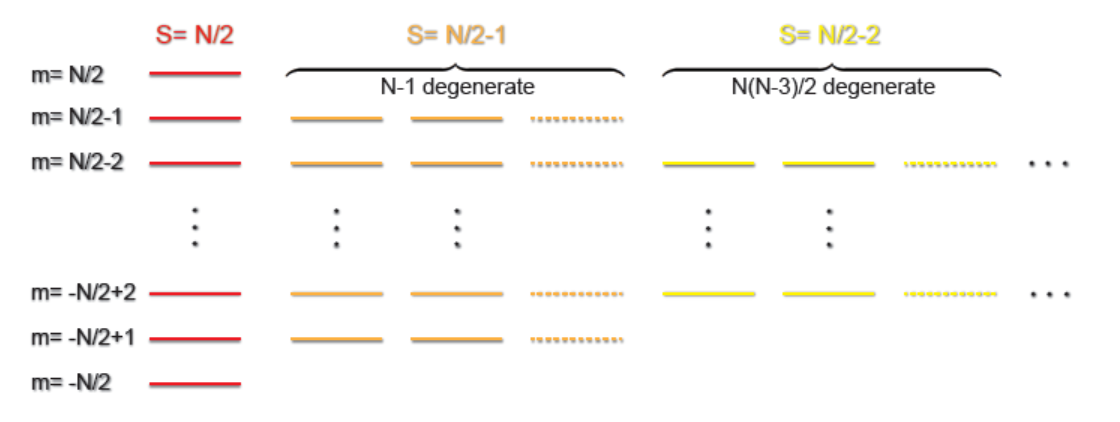
\includegraphics[width=4.5in]{NV_ensemble_levels.png}
                \caption{N个金刚石自旋构成的自旋系综的能级示意图\cite{grezes2016towards}。可以看见$\mathcal S \neq N/2 $的态均为高度简并态。}
                \label{fig:NV_ensemble_levels}
            \end{figure}




            当自旋系综从谐振腔吸收一个光子时,相应的态为$\ket B = \ket{N/2, -N/2 + 1} \equiv = \mathcal S_+ \ket G/|\mathcal S_+ \ket G| = \sum_k \ket{E_k}/\sqrt N $。其余$N-1$个单激发的激发态可写为$\ket{D_j} = \sum^{N-1}_{k=0} \exp(ijk2\pi/N)\ket{E_k}/\sqrt N $,其中$j=1,...,N-1$,且易验证$\braket{D_j|B} = 0 $。因此由能级图\ref{fig:NV_ensemble_levels}易看出所有$\ket{D_j}$对应的态均为$\mathcal S = N/2-1$,因此不可能通过$H_{TC}$与基态$\ket{G}$耦合起来。综合上述讨论,
            \begin{align}
                \bra{E,0} H_{TC} \ket{G,1} &=(1/\sqrt N)\sum_i g = g\sqrt N\\
                \bra{D_j,0} H_{TC}\ket{G,1} &= 0
            \end{align}
            
            
           通过上述计算可以看出,对于$N$个自旋构成的自旋系综,系综整体与谐振腔的耦合强度比单个自旋的耦合强度大了系数$\sqrt N$。
            

        % subsection simulation_experimental_works (end)



        \section{超导量子比特的制备与测量} % (fold)
        \label{sec:fabrication_characterization}
            
            建立超导量子比特与自旋的混合量子系统的基础之一是两者的成功耦合,以及超导量子比特的制备与调控。因此,本文也将对超导量子比特的理论基础\cite{schuster2007circuit,koch2007charge},制备方法\cite{krantz2010investigation,kelly2015fault}以及测量方法\cite{weber2016quantum}进行调研与总结,并以文献综述的形式给出。

        % subsection fabrication_characterization (end)


%!TEX root = ../main.tex
\chapter{自旋与谐振腔耦合强度仿真}
\label{cha:spin_simulation}



        通过文献综述我们看到,单个自旋与常见谐振腔的耦合强度较弱,因此我们希望通过利用自旋系综与谐振腔进行耦合或者尝试新的谐振腔设计来解决这个问题。对自旋系综与谐振腔进行耦合的情况,由于自旋系综在空间有分布,而谐振腔所产生的磁场在空间也有所分布,因此探究谐振腔产生的磁场的空间分布即成为估计耦合系数的强度大小极其空间分布的重要步骤。

        另一方面,与平面波导谐振腔相对应,三维谐振腔的电磁场空间分布更均匀,但强度相对更弱,因此耦合强度更小。在尝试更新的谐振腔设计时,我们也考虑改良三为谐振腔使之在保持自旋系综存在空间部分电磁场仍旧相对均匀的同时尽可能增加场强,而对于平面波导谐振腔,我们从进一步增大耦合强度并与单个自旋耦合的角度出发在现有提案\cite{sarabi2017prospective}的基础上进行了仿真,改进与优化。

        \section{新型3D谐振腔与自旋系综的耦合} % (fold)
        \label{sec:新型3d谐振腔与自旋系综的耦合}

        我们首先发现并重复了对优化电磁场分布均匀性的3D谐振腔的仿真\cite{Angerer2016}。这种三维谐振腔中电流与磁场分布示意图如下图所示

        \begin{figure}[h]
                \centering
            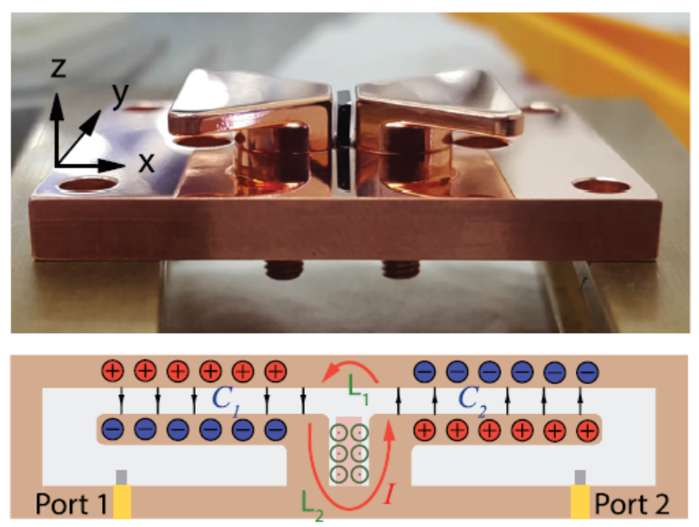
\includegraphics[width=4in]{3DResonator_image.png}
            \caption{新型三维谐振腔的几何结构与电流,磁场分布示意图\cite{Angerer2016}}
            \label{fig:3D_Resonator_image}
        \end{figure}
        其中这种三维谐振腔在普通密闭金属盒构成的三维谐振腔的基础上将电场与磁场局限于更小的体积当中,电场主要分布于两个扇形与盒顶之间,磁场主要分布于两扇形竖直支撑部分的两个平面之间,也为固定自旋系综的空间区域。因此这种三维谐振腔通过减小模式体积提高了零场涨落的大小,并同时仍保证自旋系综与磁场有较为均匀的耦合。


        \begin{figure}[h]
                \centering
            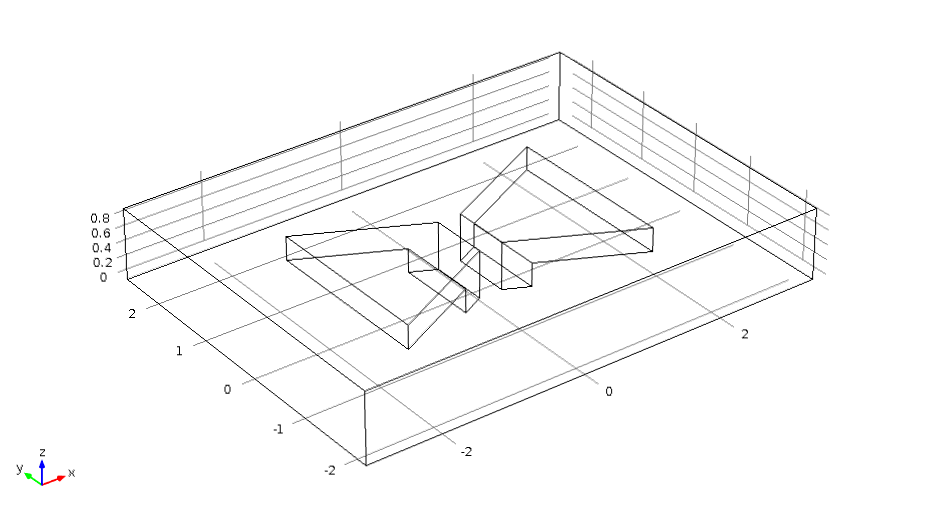
\includegraphics[width=4in]{geo.png}
            \caption{新型三维谐振腔仿真的几何设计(透视图)}
            \label{fig:geo_3DResonator}
        \end{figure}

        \begin{figure}[h]
                \centering
            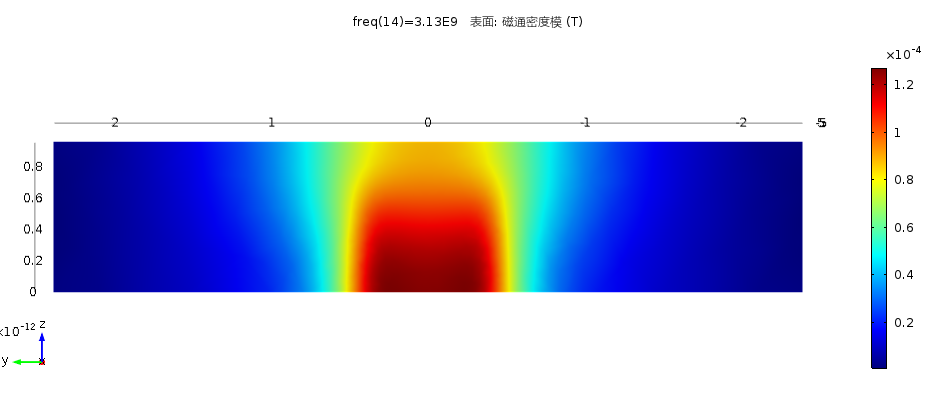
\includegraphics[width=4.5in]{normB_cross_sec_mid_yz_3.13GHz_smooth.png}
            \caption{新型三维谐振腔磁场在自旋系综所处空间横截面上的大小分布}
            \label{fig:sim_result_BField_crossSection}
        \end{figure}

        通过对Angerer等人使用的三维谐振腔的观察,我设计了如图\ref{fig:geo_3DResonator}所示几何形状的三维谐振腔。利用COMSOL求解谐振腔中电磁场的分布,能够得到自旋系综所在的横截面上的磁场分布如图\ref{fig:sim_result_BField_crossSection}所示。谐振腔的频率响应为频率和衰减率的函数\cite{grezes2016towards}
        \begin{equation}
            |S_{21}|^2 = \left | \frac{i \kappa/2}{2 \pi (\delta f - \delta f_c)+i (\kappa + \kappa_L)/2 } \right|^2
        \end{equation}
        通过对仿真所得的谐振腔的频率响应进行拟合,能够得到谐振腔的衰减率$ \kappa, \kappa_L $,进而求出对应任意功率下的谐振腔中的光子数\cite{grezes2016towards}
        \begin{equation}
            n = \frac{2 \kappa}{h f_c (\kappa+ \kappa_L)^2} P
        \end{equation}
        谐振腔中仿真的场与功率相关,知道给定功率下的谐振腔中的电磁场分布,以及相应腔内光子数后,即可简单计算得单位光子数对应的电磁场大小与分布。通过单位光子数的磁场大小,即可计算自旋与谐振腔中该模式的耦合强度\cite{Angerer2016}
        \begin{equation}
            |g_0| = \sqrt{\frac{2}{3}} \frac{\mu_B g_e}{2\hbar} |\bm B_0||\bm S| \sim 100 \mathrm{mHz}
        \end{equation}

        通过仿真,拟合与计算得到的耦合强度,与Angerer等人所得到的耦合强度的数量级相符,验证了我们的仿真与计算的正确性。综合考虑后,我们认为这种方法对耦合强度的增加不明显,没有数量级的提升,并且这种三维谐振腔的制备较为复杂,我们没有继续进行这种新型三维谐振腔的制备。
        
        
        





        \section{2D平面波导谐振腔与自旋系综的耦合} % (fold)
        \label{sec:2d平面波导谐振腔与自旋系综的耦合}

        目前有很多工作通过将自旋系综与二维平面波导谐振腔进行耦合,达到了强耦合的效果\cite{kubo2010,Schuster2010}。对于这类耦合,谐振腔的耦合强度的大小及其分布依赖于电磁场的空间分布。因此,我对二维平面波导的电磁场的空间分布进行了仿真,并与文献进行了比较。

        对于二维平面波导的仿真,空间中场的分布由金属中电流密度的分布决定,因此仿真的关键为得到可靠的电流密度分布,从而得到空间中场的分布。超导效应对金属中场的分布体现在电流穿透金属表面的深度有限,即与高频电流导致的趋肤效应十分类似,因此可通过高频电流的趋肤效应对超导电流的分布进行模拟\cite{Mark2013}。趋肤效应的深度电流频率相关:
        \begin{equation}
            \lambda_{skin} = \sqrt{\frac{2}{\sigma \omega \mu}}
        \end{equation}
        通过使趋肤效应的深度等于超导电流的穿透深度,我们估计得仿真所需采用的电流频率为$ \omega \approx 660 $GHz。这个频率并不对应实际物理系统中的任何频率,仅为仿真所采用的一个参数。零场涨落下的电磁场分布直接通过使总电流的大小为零场电流涨落的大小来得到。零场电流的大小通过计算可得\cite{PhysRevA.95.022306,Mark2013,Tosi2014}
        \begin{align}
            \label{eqn:ZPF_estimation}
            \frac{\hbar \omega }{2} &= 2\times \frac{1}{2}L (\delta i_{rms})^2\\
            L&= \frac{2Z_0}{\pi \omega}\\
            \delta i_{rms } &= \omega \sqrt{ \frac{\hbar \pi}{4Z_0} }\approx 50 \mathrm{nA}
        \end{align}
        
        通过上述方法,我采用了与两篇文章中相同的器件几何尺寸对磁场进行了仿真,如图所示。


        \begin{figure}
            \begin{minipage}[b]{0.4\textwidth}
                \centering
                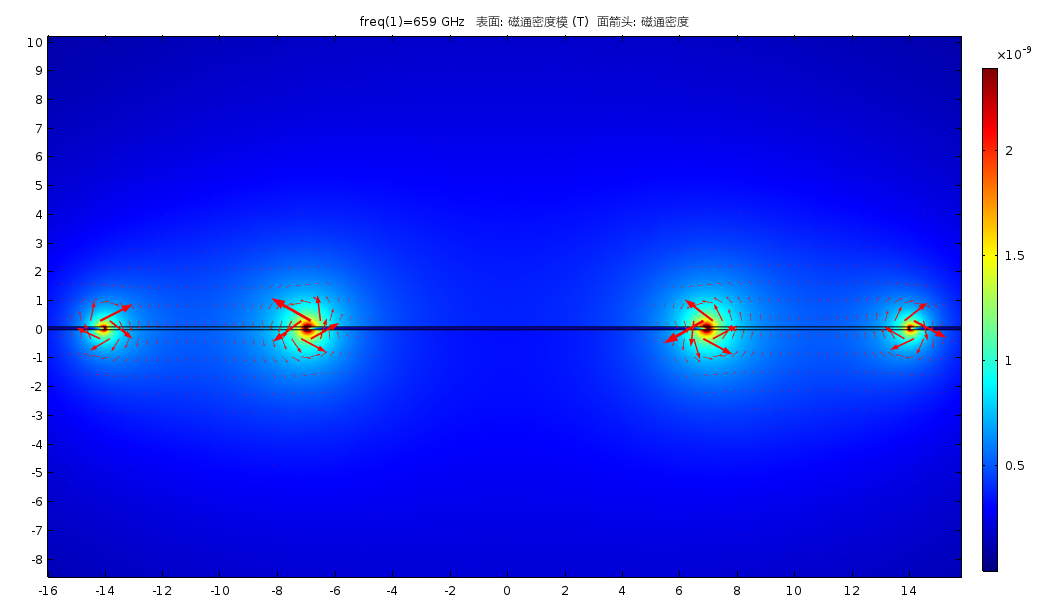
\includegraphics[width=3in]{20161122_Bnorm_cross_659GHz.png}
                \caption{仿真所得磁场空间分布截面图}
                \label{fig:20161122_Bnorm_cross_659GHz}
            \end{minipage}%
            % \hspace{0.1\textwidth}%
            % \hfill
            \hspace*{\fill}
            \begin{minipage}[b]{0.5\textwidth}
                \centering
                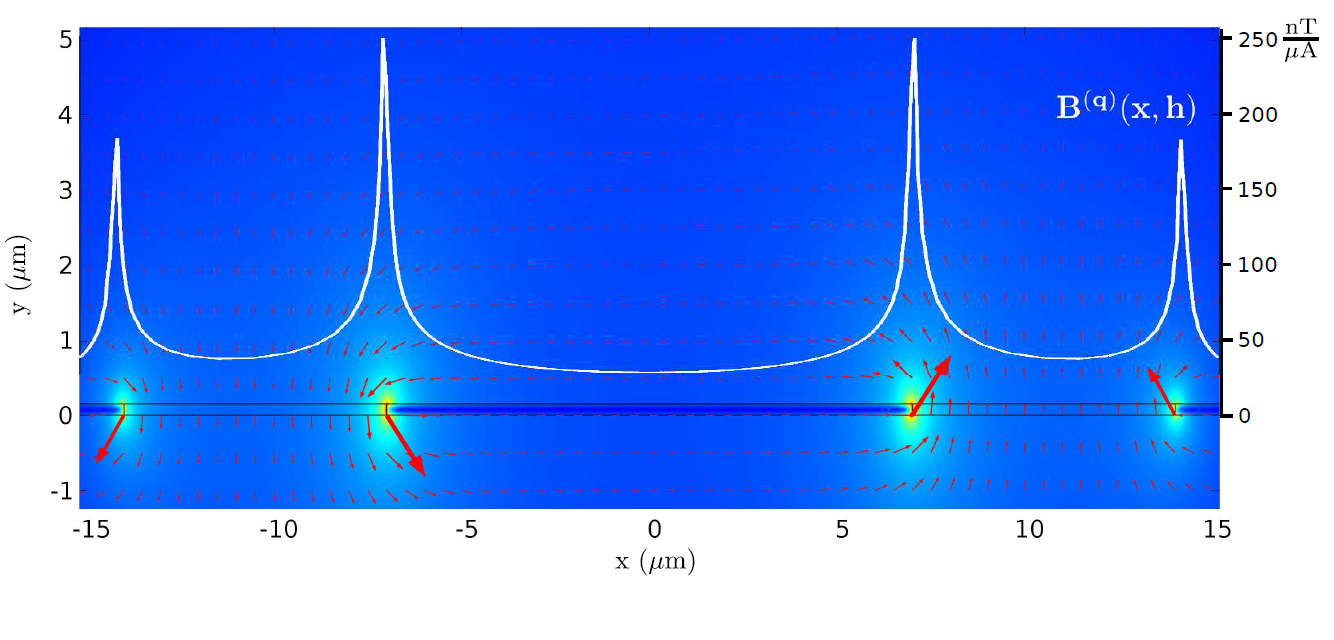
\includegraphics[width=3.5in]{Coupling-SMM-to-quantum-circuits-fig7.png}
                \caption{文献\cite{Mark2013}中所示磁场空间分布截面图}
                \label{fig:Coupling-SMM-to-quantum-circuits-fig7}
            \end{minipage}
        \end{figure}
        
        \begin{figure}
            \begin{minipage}[b]{0.4\textwidth}
                \centering
                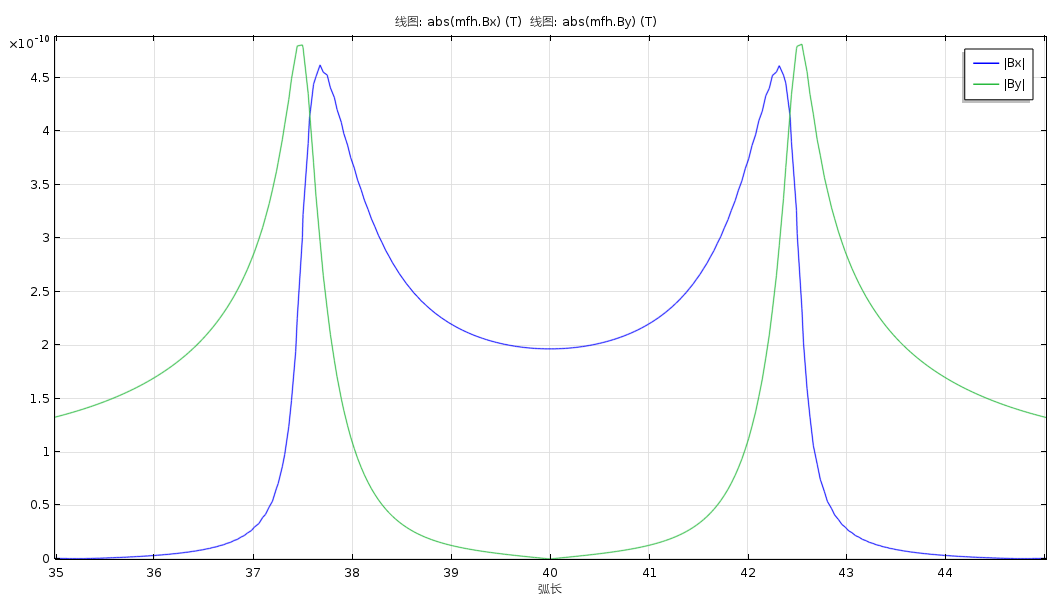
\includegraphics[width=3in]{20161122-2_Bxy_0.1um_below_659GHz.png}
                \caption{仿真所得磁场在位于距金属上表面$0.1\mu m$处水平截线上的分布}
                \label{fig:20161122-2_Bxy_0.1um_below_659GHz}
            \end{minipage}%
            % \hspace{0.1\textwidth}%
            % \hfill
            \hspace*{\fill}
            \begin{minipage}[b]{0.5\textwidth}
                \centering
                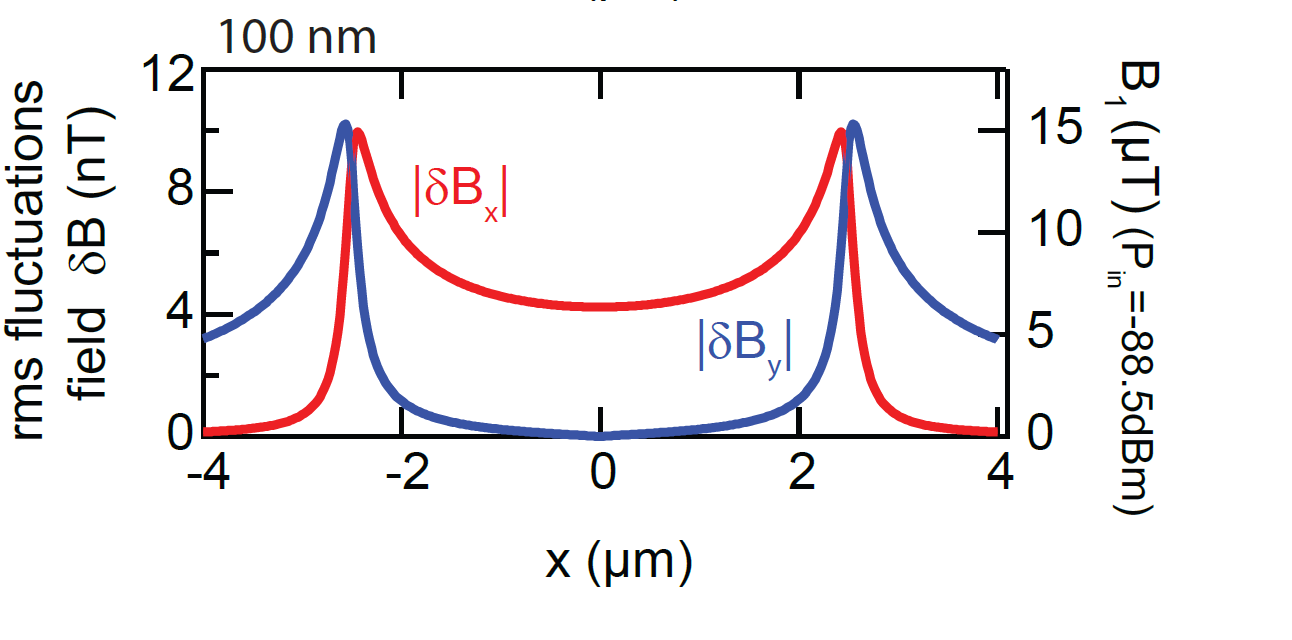
\includegraphics[width=3.5in]{Reaching-the-quantum-limit-of-sensitivity-SI-fig3d.png}
                \caption{文献\cite{Bienfait2016a}中所示磁场在位于距金属上表面$0.1\mu m$处水平截线上的分布}
                \label{fig:Reaching-the-quantum-limit-of-sensitivity-SI-fig3d}
            \end{minipage}
        \end{figure}
        

        通过利用上述方法对两篇独立的文章中的几何结构进行仿真并且与文章中的结果比较,可以看出结果相符。验证上述方法的可行性后,我对我们制备的二维平面波导的常见几何尺寸进行了仿真,并绘制了距离波导金属表面不同高度处的水平截线上的磁感应强度分布,如图\ref{fig:20161122-2_Bnorm_lines_659GHz}所示。

        \begin{figure}[h]
                \centering
            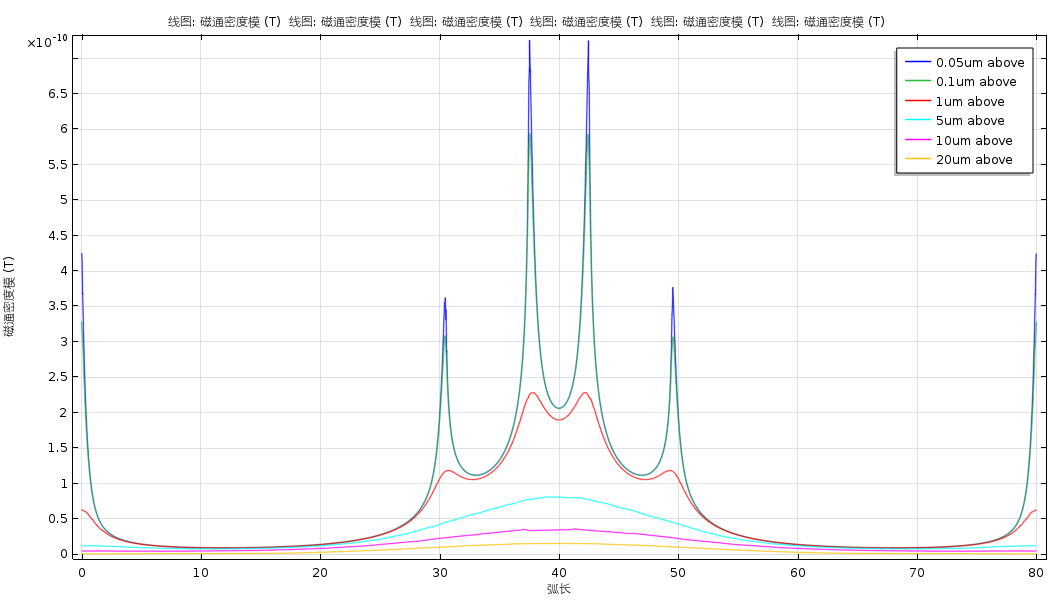
\includegraphics[width=4.5in]{20161122-2_Bnorm_lines_659GHz.png}
            \caption{基于我们制备的二维平面波导的常见几何尺寸进行仿真所得的磁感应强度分布图。}
            \label{fig:20161122-2_Bnorm_lines_659GHz}
        \end{figure}

        通过仿真结果可以看出,磁场在金属上方$10 \mathrm{\mu m}$左右的范围内开始分布均匀,并且强度在$ 0.5\times 10^{-10} $T的范围左右,对应的耦合强度$ g \sim 2 \pi \cdot 10 $Hz,与文献中对单个自旋与二维平面波导谐振腔的耦合常数的估计值相符很好。因此,通过这种仿真方法,我们能够很快得到给定任意几何形状的二维平面波导的空间磁场分布,进而得到空间内任意一点处的自旋与基于该二维平面波导构成的谐振腔的模式的耦合强度。







        \section{螺旋状电感谐振腔与2.5维谐振腔与单个自旋的耦合} % (fold)
        \label{sec:螺旋状电感与2_5d谐振腔与单个自旋的耦合}

            前面讨论了利用与自旋系综耦合来增大耦合常数。通过观察耦合常数的表达式\ref{eqn:coupling_coeff},可以看见还可以通过提高零场涨落的大小来提高单个自旋与谐振腔模式的耦合常数。


            \subsection{参数估计} % (fold)
            \label{sub:参数估计}

                通过对零场电流大小进行估计的\ref{eqn:ZPF_estimation}式,可以看到零场电流涨落
                \begin{equation}
                    \delta I = \sqrt{ \frac{\hbar \omega}{2 L} }
                \end{equation}
                而对于选定的自旋种类以及基于选定自旋的能级系统定义出的二能级量子比特,其能级间能量差大致固定,因此谐振腔的谐振频率也大致固定在该能量所对应的频率。而谐振腔的频率由$ \omega = 1/\sqrt{LC} $确定。通过上述讨论可以看到,通过增大零场电流涨落可以增大磁场,进而增大单个自旋与谐振腔模式的耦合常数,增大零场电流涨落可由减小谐振腔的电感$L$实现,而对于固定频率的谐振腔,减小$L$意味着增大电容$C$。如果我们想要达到的耦合强度$ g/2 \pi \sim 1 \mathrm{MHz} $,并且利用如基于金刚石色心的能量差对应频率在$3 \mathrm{GHz} $左右的自旋系统,可以估计出相应的零场电流涨落,对应的谐振腔电感与电容的数量级为
                \begin{align}
                    \delta I & \sim  1 \mathrm{\mu A}\\
                    L & \sim  1 \mathrm{pH}\\
                    C & \sim  1 \mathrm{nF}
                \end{align}
                对于nF数量级的电容,无法通过如齿状二维电容等二维设计实现,而可使用三维平板电容实现。因此,我把这种电感为二维结构而电容为三维结构的谐振腔称为2.5维谐振腔。已有研究人员提出基于这种思路设计的2.5维谐振腔\cite{sarabi2017prospective},我基于他们的谐振腔设计进行了仿真与优化。
                

                
            \subsection{电感设计与优化} % (fold)
            \label{sub:电感设计与优化}

                Sarabi等人提出的设计如图\ref{fig:spiral_proposal_1}所示


            \begin{figure}
                \begin{minipage}[b]{0.4\textwidth}
                    \centering
                    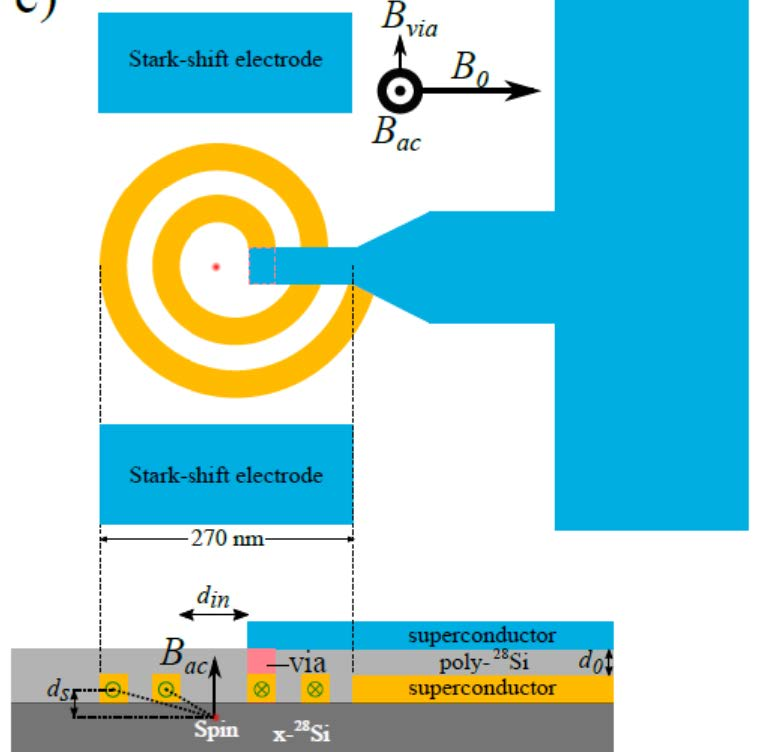
\includegraphics[width=3in]{spiral_proposal_1.jpg}
                    \caption{来自参考文献~\inlinecite{sarabi2017prospective}的2.5维谐振腔的设计(右图中红色虚线部分的局部放大图)。}
                    \label{fig:spiral_proposal_1}
                \end{minipage}%
                % \hspace{0.1\textwidth}%
                % \hfill
                \hspace*{\fill}
                \begin{minipage}[b]{0.5\textwidth}
                    \centering
                    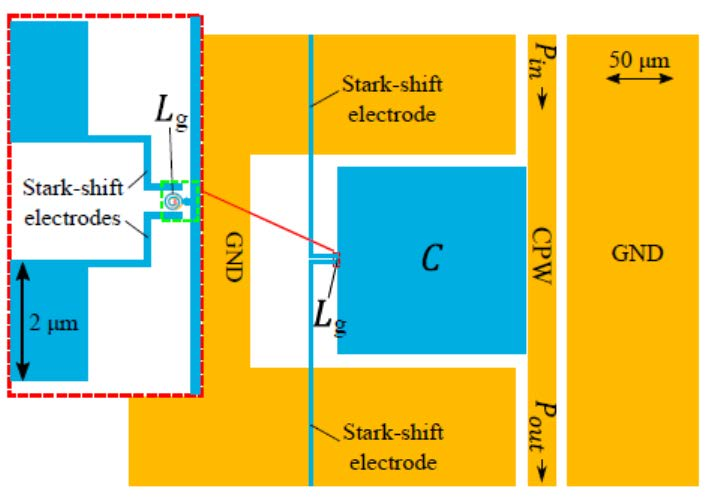
\includegraphics[width=3.5in]{spiral_proposal_2.jpg}
                    \caption{来自参考文献~\inlinecite{sarabi2017prospective}的2.5维谐振腔的设计(整体)。}
                    \label{fig:spiral_proposal_2}
                \end{minipage}
            \end{figure}
            其中主要图示均为俯视图,左图的下方的小图为横截面示意图。右图中蓝色的部分即为层状电容的俯视图。通过根据相关几何参数进行仿真,我得到了这种谐振腔的电感部分的磁场分布图,如图\ref{fig:res_spiral_normB_xy_20170314}所示。通过分析我们发现,耦合系数能够得到数量级上的提升的根本原因是选取了很小的电感$L$,从而得到了较大的零场磁场涨落,并且自旋距离电感部分导线的距离较近,为$~10$nm的数量级。而与之相对的,螺旋状电感的螺旋圈数则相对不那么重要,不会对耦合强度产生数量级上的影响,反而加大了微纳加工制备的难度。因此,我们进一步对螺旋状电感进行了分析,改良与仿真。

            \begin{figure}[h]
                \centering
                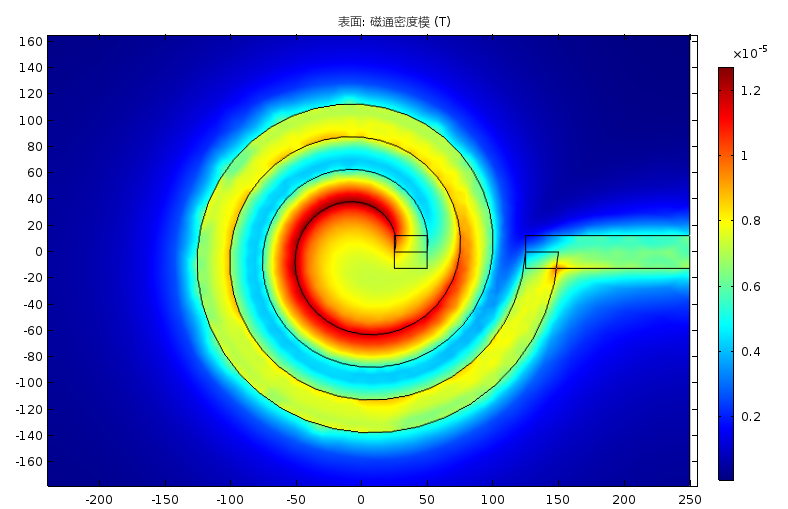
\includegraphics[width=4in]{res_spiral_normB_xy_20170314.png}
                \caption{2.5维谐振腔的螺旋状电感处水平截面上的磁感应强度分布。}
                \label{fig:res_spiral_normB_xy_20170314}
            \end{figure}

            \begin{figure}[h]
                \centering
                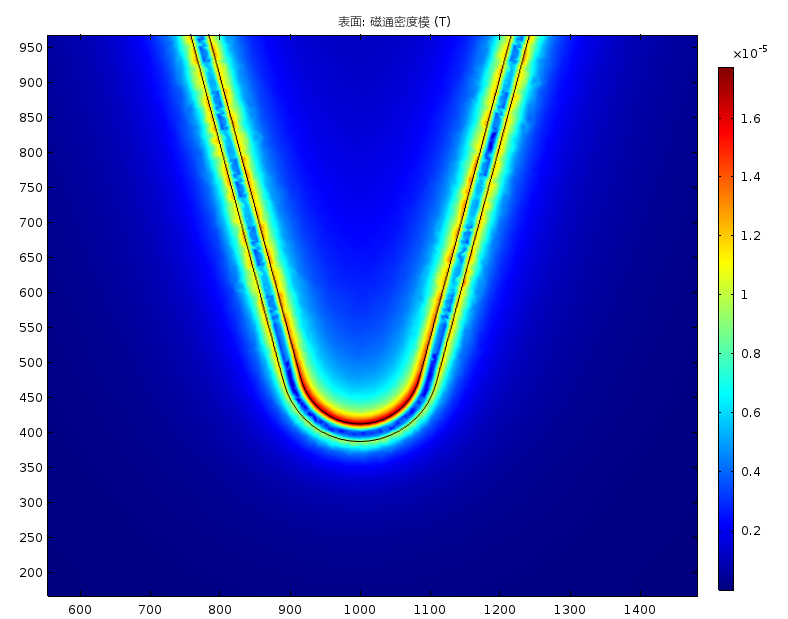
\includegraphics[width=3in]{res_UInd_normB_20170317.png}
                \caption{第一次改进后的2.5维谐振腔的电感处水平截面上的磁感应强度分布。}
                \label{fig:res_UInd_normB_20170317}
            \end{figure}


            \begin{figure}[h]
                \centering
                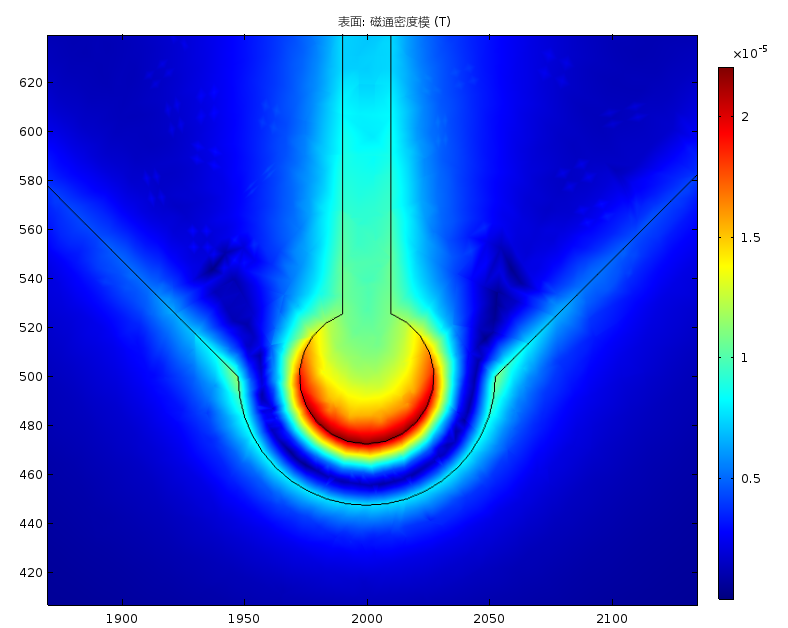
\includegraphics[width=3in]{res_UIndV3_normB_20170321.png}
                \caption{第二次改进后的2.5维谐振腔的电感处水平截面上的磁感应强度分布,电感部分的电感大小得到了降低。}
                \label{fig:res_UIndV3_normB_20170321}
            \end{figure}

            

            \begin{figure}[h]
                \centering
                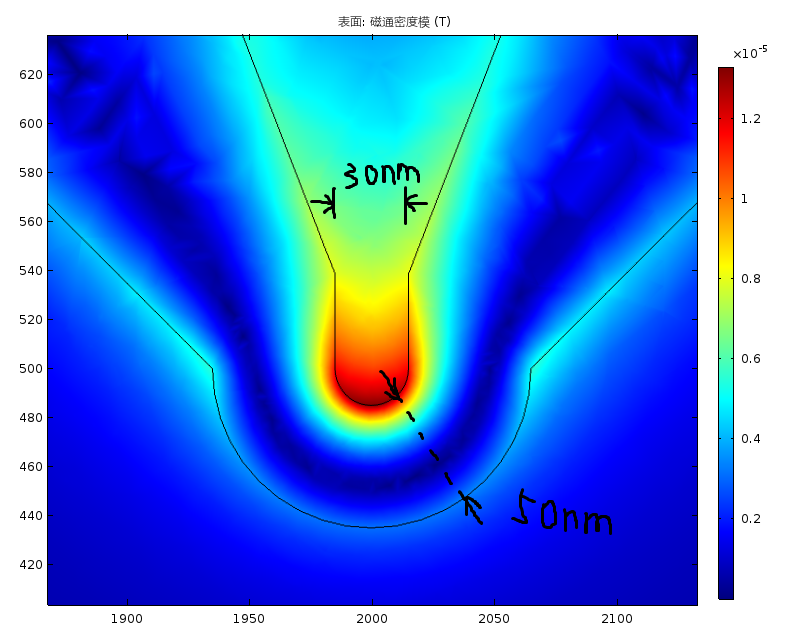
\includegraphics[width=3in]{res_UIndV4_50nm_normB_20170406.png}
                \caption{第三次改进后的2.5维谐振腔的电感处水平截面上的磁感应强度分布,通过加厚材料并加粗宽度提升了临界电流大小,并在不影响磁场较强区域的强度的基础上改进了设计以提高制备的成功率。}
                \label{fig:res_UIndV4_50nm_normB_20170406}
            \end{figure}


            首先,我简化了螺旋状的电感结构,直接采用一根细导线作为电感,并通过磁场仿真来估算电感的数量级,仿真结果如图\ref{fig:res_UInd_normB_20170317}所示。通过仿真估算得到的电感值为$L\approx 2\times 10^{-12} \mathrm{H} $,比理想的电感值多出一倍左右。考虑到所需的强磁场区域并不需要分布于整个电感导线,而只需要在圆弧附近即可,而强磁场存在的区域更大自然会增大导线的自感。基于这个想法,我进一步改进了电感的几何设计,仅保留电感中间的圆弧部位较细,这样电流密度增大,磁场相应增大,而对于电流流入与流出圆弧部位的部分,使导线变宽,如图\ref{fig:res_UIndV3_normB_20170321}所示,即可减小大部分区域的磁场大小。通过仿真得出,电感大小的确减小到$L \approx 7\times 10^{-13} \mathrm{H} $,减小超过50\%。

            通过进一步讨论并考虑到测量系统的温度下限对应的噪声大小,我们希望谐振腔中能有远多于100个光子的信号。通过简单估计我们发现对于图\ref{fig:res_UIndV3_normB_20170321}以及其之前的结构,达到理想的光子数会使电流密度超过所用材料的超导临界电流密度,这样极有可能使器件损耗大大增加,并且因非超导态的电阻发热使电感部分的细导线烧断,导致器件损毁,因此需要进一步改进设计使同样临界电流密度的材料能够承载更多的电流。另一方面,图\ref{fig:res_UIndV3_normB_20170321}的设计由于电感环状结构的前后为尽可能增大导线宽度使输入与输出导线中部距离十分靠近,为$\sim 10 \mathrm{nm} $的数量级,在微纳加工过程中极易连接起来,在实际测试中也出现输入与输出两部分连接起来的现象。考虑上述两个因素后,我进一步改进了电感的设计,通过加厚材料并加宽导线圆弧部分,提高了可承载总电流的大小,并使导线的输入与输出部分分离更远距离,提高了制备的成功率。最终的电感设计如图\ref{fig:res_UIndV4_50nm_normB_20170406}所示。

            
            对于COMSOL仿真所得电感的准确度,我通过变化求解空间区域大小与网格致密程度,以及与经验公式相比较这两种方法进行了探究。对于矩形截面的直导线,其自感的计算公式为\cite{grover2004inductance}

            \begin{equation}
                \label{eqn:SelfInductance}
                L = 0.002l \left [ \ln \frac{2l}{B+C} + \frac{1}{2} - \ln(e) \right ]
            \end{equation}
            其中$B$,$C$为导线矩形横截面的边长,$l$为导线的长度,以厘米为单位,这样计算出的电感的单位为$ \mu  $H。最后一项$\ln(e)$并不等于一,需查表得知,但其值基本为$0.001$,对于当前的估计的精度而言可以忽略。
            

            通过仿真几何结构为20nm~x~20nm~x~250nm的直导线的自感,不同求解区域大小下COMSOL计算所得的电感值以及经验公式估计所得的电感值如表\ref{tab:InductanceComparison}所示。


\begin{table}[htb]
  \centering
  \caption{不同大小求解区域下COMSOL仿真所得电感值与经验公式估计的电感值}
  \label{tab:InductanceComparison}
    \begin{tabular}{c|cccc} %{\linewidth}{lX}
      \toprule %[1.5pt]
      求解区域 & $250^2\times 250$nm$^3$ & $500^2\times 250$nm$^3$ & $1000^2\times 250$nm$^3$ & 经验公式 \\
      \midrule %[1pt]
      电感值(H) & $1.378\times 10^{-13} $ & $1.705\times 10^{-13} $ & $2.019\times 10^{-13} $ & $1.512\times 10^{-13} $  \\
      \bottomrule %[1.5pt]
    \end{tabular}
\end{table}

        
        从表\ref{tab:InductanceComparison}中可以看出,COMSOL仿真的电感值随求解区域有较明显变化,但能够得到与经验公式数量级相符的结果。实际使用的电感也较为复杂,通过COMSOL的仿真与经验公式的估算也仅能给出一个参考值,具体还需通过实际制备出的器件积累数据与经验。

    
%!TEX root = ../main.tex

        \chapter{PPMS测量系统} % (fold)
        \label{cha:PPMS测量系统}
            器件的测量在PPMS(Physical Proerty Measurement System)中进行,为基础的二端微波测量。在PPMS中器件被冷却到2K左右,此时金属Nb进入超导态。通过网络分析仪直接测量二维平面波导的透射信号,即可在谐振腔的谐振频率处看到透射信号被吸收形成的凹陷。我利用现有的其他类型谐振腔对测量系统进行了测试,并通过拟合可得到谐振腔的相关参数。在测量系统搭建较为完善的基础上,进一步进行2.5维LC谐振腔的测量。

            \section{测量系统概述} % (fold)
            \label{sec:测量系统概述}

            实验中使用的网络分析仪为Agilent Technologies E5071C ENA series network analyzer,输出频率范围为300kHz至20GHz,下文中将简称其为VNA。


        \begin{figure}[h]
                \centering
            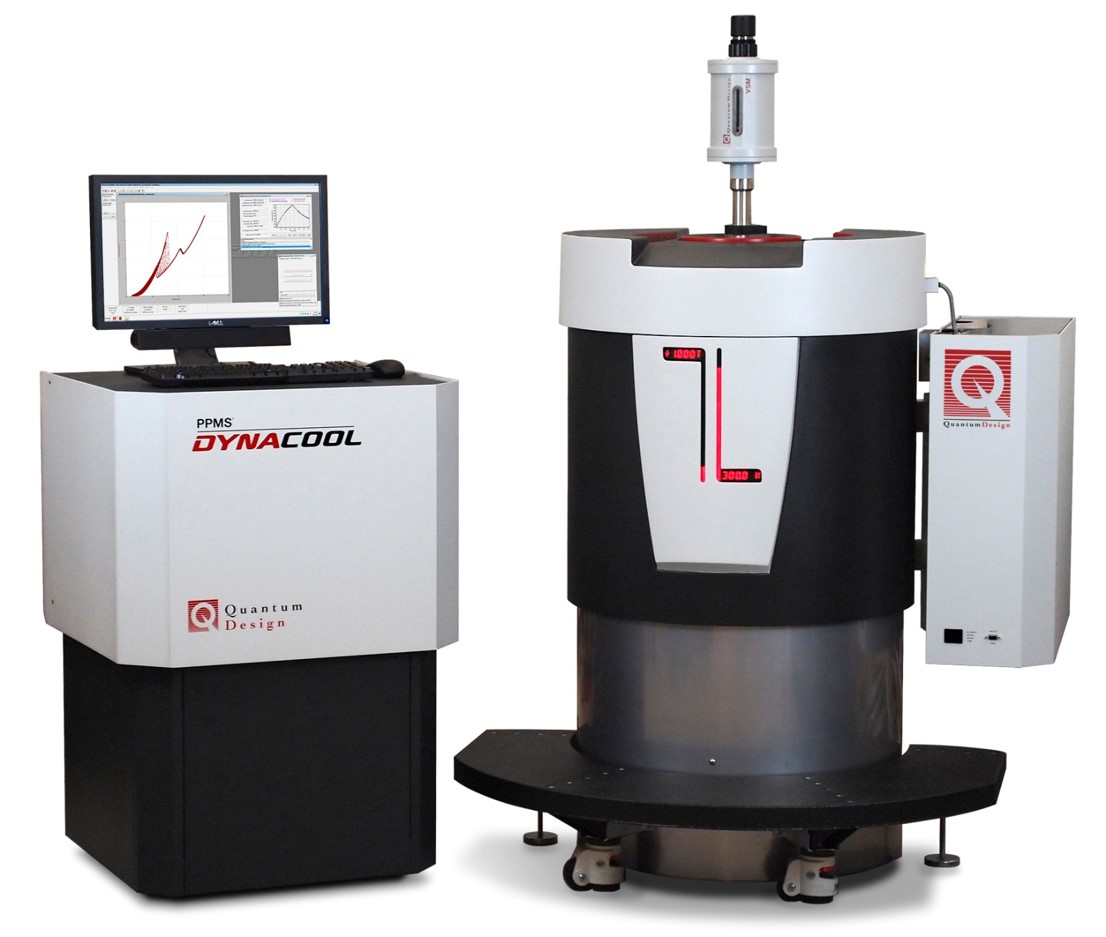
\includegraphics[width=4in]{DynaCool.jpg}
            \caption{PPMS DynaCool测量设备实物图\cite{QDDynaCool}}
            \label{fig:DynaCool}
        \end{figure}

            实验中所用的PPMS为QuantumDesign公司的DynaCool\cite{QDDynaCool},本文中都将简称它为PPMS。该PPMS可降温至1.8 K,加磁场最大为9T或14T,取决于磁体的型号。PPMS本体如图\ref{fig:DynaCool}所示,主要由控制电脑与仪器腔体两部分组成。仪器腔体的内部结构由图\ref{fig:DynaCoolStructure}所示。该图为仪器腔体在竖直平面内的横截面,可以看见样品室为被制冷环境包围住的一个立体圆柱形结构,直径不到一分米,有效的温度与磁场区域的高度大概在一分米左右。


        \begin{figure}[h]
                \centering
            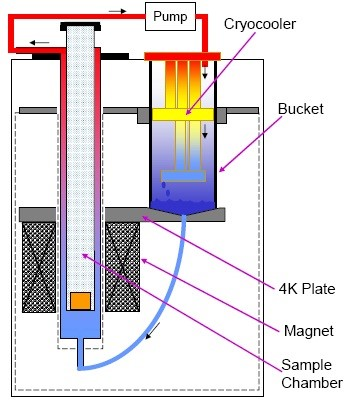
\includegraphics[width=4in]{PPMSStructure.jpg}
            \caption{PPMS DynaCool腔体内部结构\cite{QDDynaCool}}
            \label{fig:DynaCoolStructure}
        \end{figure}

            由于测量样品所在区域较小,因此无法进行需要很多端口的微波测量,但对于测量谐振腔性质所需的两个端口甚至一个端口来说较为合适。通过减小样品空间所取得的优点即在于,该PPMS系统的制冷系统长时间处于4K的低温,样品位于相对独立的样品室中,通过样品架与制冷系统的物理接触达到降温的效果,因此样品室可以较快地升温降温,而不需要对整个制冷系统进行升温降温。实际使用过程中,升温过程与降温过程所需时间均仅为30分钟左右,使得更换样品极为便捷。



            在开始本文的测量相关项目之前,该PPMS系统多用于直流测量,没有微波测量所需的设备。该部分设备的改造由交叉信息研究院孙麓岩研究组的郭星翰同学完成。改装后的样品通过样品托固定于样品杆上,进而通过样品杆插入PPMS的样品室中。由郭星翰设计的样品托如图\ref{fig:samplerodHolder}中蓝色矩形部分所示,由底座与盖子两部分组成。更换器件时,首先使PPMS样品室回到常温常压,取出样品杆,将样品托底座从盖子上拆下,再将旧样品从底座上取下,新样品安装上底座后将底座装回,插回样品杆即可。如图\ref{fig:samplerodHolder}所示,所测量的器件大小为4mm~x~7mm,放置于样品盒底座上的PCB板中央,通过点焊与PCB板相连。PCB板上焊接有两个SMP接头,与样品杆上的微波线相连并接入VNA的输入与输出端口。


\begin{figure}[h]
  \centering%
  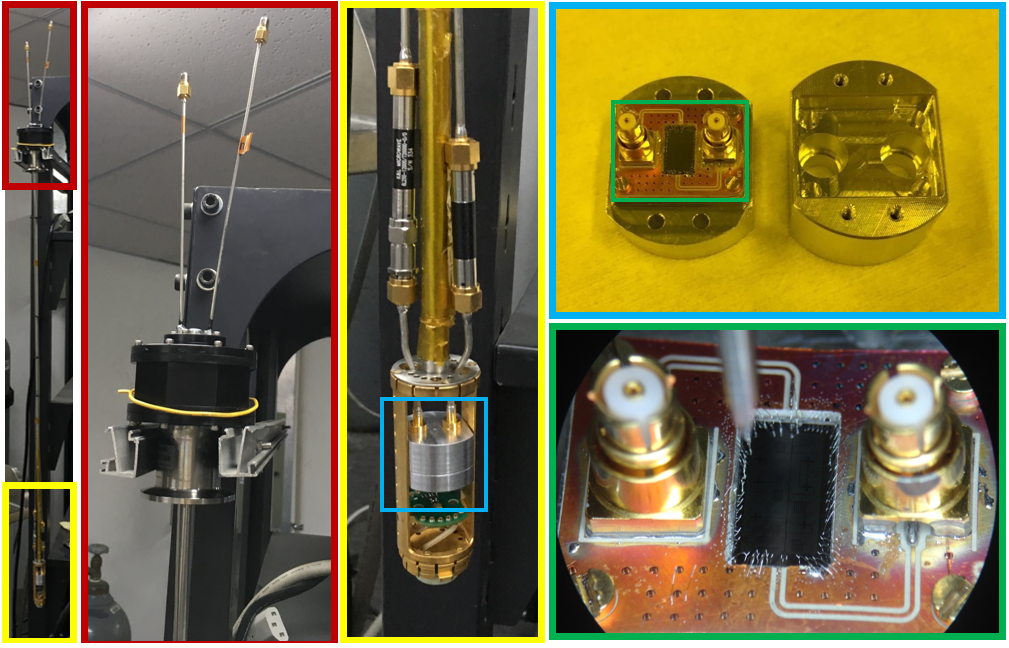
\includegraphics[width=5in]{SampleRodAndHolder.png}
  \caption{样品杆与样品盒。其中红色矩形部分为样品杆末端微波信号的输入与输出端,黄色矩形部分为样品盒所处位置,蓝色矩形为样品盒以及拆卸后的样品盒。}
  \label{fig:samplerodHolder}
\end{figure}

            在实验进行过程中,我们考虑到将来进行自旋与谐振腔耦合的相关实验时需要加入竖直方向的磁场以改变自旋能级间距,而现有设计下磁场垂直与器件表面,对超导态下的器件的性质影响较大。因此,我在现有样品托的基础上改进了样品托底座与盖子以及PCB板的设计,具体在第\ref{sec:样品托的设计与优化}节中详细进行描述。
                
            % section 测量系统概述 (end)

            \section{测量系统的程序编写} % (fold)
            \label{sec:测量系统}
            通过VNA测量谐振腔的频率响应时,需要调整VNA的输出功率,IFBW,扫描频率范围,平均次数等一系列参数。这些调整步骤既可通过仪器前面板的按钮进行,也可通过远程通讯来控制。考虑到测量的便捷性,我希望通过GPIB线与VNA进行通讯并取得数据。通过Agilent提供的GPIB-USB转接头建立硬件连接,并安装Keysight Instrument Control Bundle软件后,转接头上的工作指示灯正常。Keysight Instrument Control Bundle软件提供了Keysight IO Libraries Suite软件的安装与Command Expert软件的安装。前者能够方便地查看仪器的连接状态,后者则提供仪器的SCPI指令集并可测试通过指令控制仪器。

            通过电脑与VNA建立通讯后,我以MATLAB提供的visa类为基础,通过Command Expert对VNA的相关控制指令进行了测试后,编写了通过MATLAB控制VNA的代码,具体代码可在附录\ref{cha:measurement_code}中查看。对于能够简单进行更改与询问的参数,重载了MATLAB的get与set方法。对于大范围的精细的扫描,编写了manualSweep方法,可自动将扫描范围分段进行,并返回最终扫描结果。对于数据处理环节,我将拟合相关的代码也整合进入测量阶段,进而能够节省重新导入数据的过程直接快速得到拟合结果。使用MATLAB代码进行谐振腔的测量,在1个小时内即可完成大范围搜索谐振腔的共振频率位置,对不同频率的谐振腔进行细扫并拟合得到品质因子这一系列实验步骤。以下为一部分示例代码。大部分代码采用了inputParser处理输入参数,使程序规范且易于理解。

            \begin{lstlisting}
% Example of using class E5071C
vna = E5071C('address',6);	% initialize the instrument object with GPIB address 6
vna.plotTrace;				% fetch current trace on VNA and plot in a figure
vna.freqCenter				% query and display the center frequency
vna.freqSpan = 10e6;		% set the frequency span to 10MHz
[freqs, trace] = vna.manualSweep('start',1e9,'stop',10e9,'res',1e5);	% manual sweep from 1GHz to 10GHz with 0.1MHz resolution
vna.freqCenter = 3.021e9;	% set frequency center
vna.freqSpan = 1e6;			% set frequency span
vna.plotTrace('issavedata',true,'avg',10);	% wait for 10 averages and save data while fetching the trace
vna.fit('fitall',true);		% fit the data in the current figure
            \end{lstlisting}



            对于PPMS的控制,仪器商为这台仪器提供了配套的LabVIEW程序,可以通过.NET网络协议远程控制PPMS。仪器商所提供的LabVIEW程序基于一个动态链接库文件QDInstrument.dll实现控制功能。为了通过MATLAB控制PPMS,我尝试将LabVIEW程序的VI封装成dll文件,再通过MATLAB加载与调用其中的函数。但由于LabVIEW的单个VI都会首先与PPMS建立连接,因此导致MATLAB中每调用一次PPMS的状态查看或是设置函数,就会重新建立一次连接,使程序运行缓慢,并且导致多个client同时与PPMS控制电脑上的server保持连接,可能导致潜在的问题。综合考虑后,我决定直接调用仪器商编写LabVIEW程序所调用的dll文件。

            由于不清楚QDInstrument.dll文件中程序的构成与相关接口,而这些信息是调用其中的函数所必需的。通过查询,我使用了ILSpy对该dll文件进行了反编译,结合LabVIEW程序对该dll的使用方法,确定了在MATLAB中正确调用该dll文件的方法,并以它为基础编写了通过MATLAB控制PPMS程序的代码。需要注意的是,在MATLAB中的PPMS代码的构造函数中我一添加了加载该动态链接库的MATLAB指令,但每次重启MATLAB后初始化一个PPMS实例时总是会遇到MATLAB无法找到或识别dll中应有的命名空间的错误。目前较为确定的解决办法是每次重新启动MATLAB时,需在命令行(Command Line)中手动通过NET.addAssembly方法加载dll文件,随后初始化PPMS实例。这时MATLAB仍然会报错,但此时尝试手动在命令行中输入相关内容,通过使用TAB键能够发现MATLAB已经能够识别出dll中的内容。这时再初始化PPMS实例仍然会得到报错,必须在命令行中输入调用dll中的任意对象,比如输入\mcode{QuantumDesign.QDInstrument.QDInstrumentType.DynaCool}后回车,随后再初始化PPMS实例即可成功。以下为加载dll与控制PPMS的代码示例,完整的PPMS控制代码附在\ref{sec:ppms控制代码}中。

            \begin{lstlisting}
% Example of using class PPMS
NET.addAssembly('path\to\the\file.dll');	% load the dll
ppms = PPMS;				% This will get error message. See the constructor for more parameters
QuantumDesign.QDInstrument.QDInstrumentType.DynaCool; % nothing happened, but required
ppms = PPMS;				% This time it should work
ppms.temp					% query and print the temperature
ppms.field					% query and print the magnetic field
ppms.tempStatus				% query the temperature status. It will return a QuantumDesign.QDInstrument.TemperatureStatus object
ppms.tempStatusStr			% query the temperature status. It returns a string, such as 'Chasing', 'Stable', etc.
ppms.fieldStatus
ppms.fieldStatusStr			% similar as for temperature status
ppms.setTemp(300,'tempRate',10,'tempApproach','FastSettle');		% set temperature
ppms.setField(1000,'fieldRate',100,'fieldApproach','Linear');		% set field
            \end{lstlisting}

            有了以上测量程序的编写,即可完全通过测量电脑询问与控制PPMS的温度与磁场,以及调节VNA的相关参数并取得VNA的扫描数据。更进一步的,通过Windows的远程桌面可以远程连接到测量电脑,从而使测量变得更为便捷。实际中我们只需要在取出和放入样品时到PPMS设备附近,其余时间均远程进行控制与测量。


            \section{样品托的设计与优化} % (fold)
            \label{sec:样品托的设计与优化}



\begin{figure}[h]
  \centering%
  \begin{subfigure}{0.4\textwidth}
    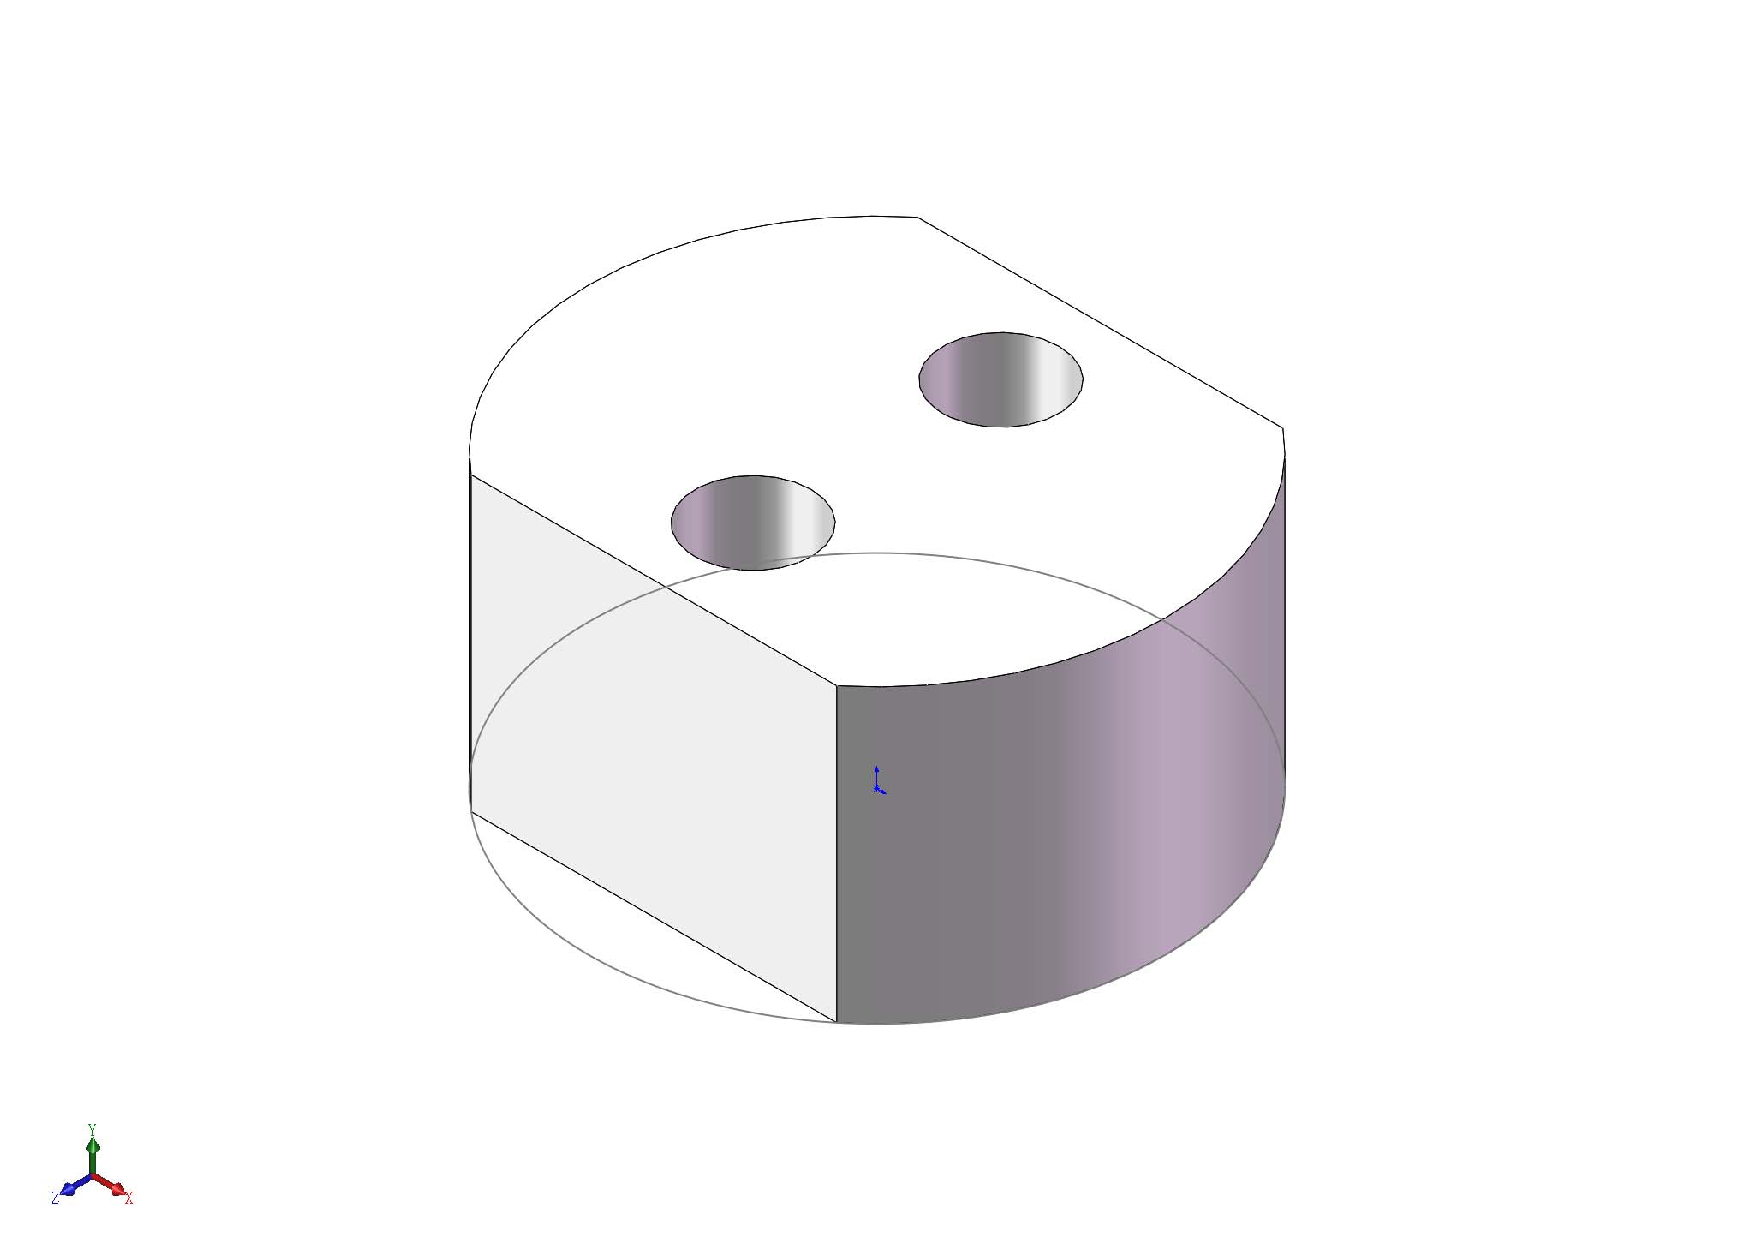
\includegraphics[width=2.2in,angle=270]{Smallbox1.pdf}
    % \caption{第一个小图形}
  \end{subfigure}%
  % \hspace{4em}%
  \hfill
  \begin{subfigure}{0.4\textwidth}
    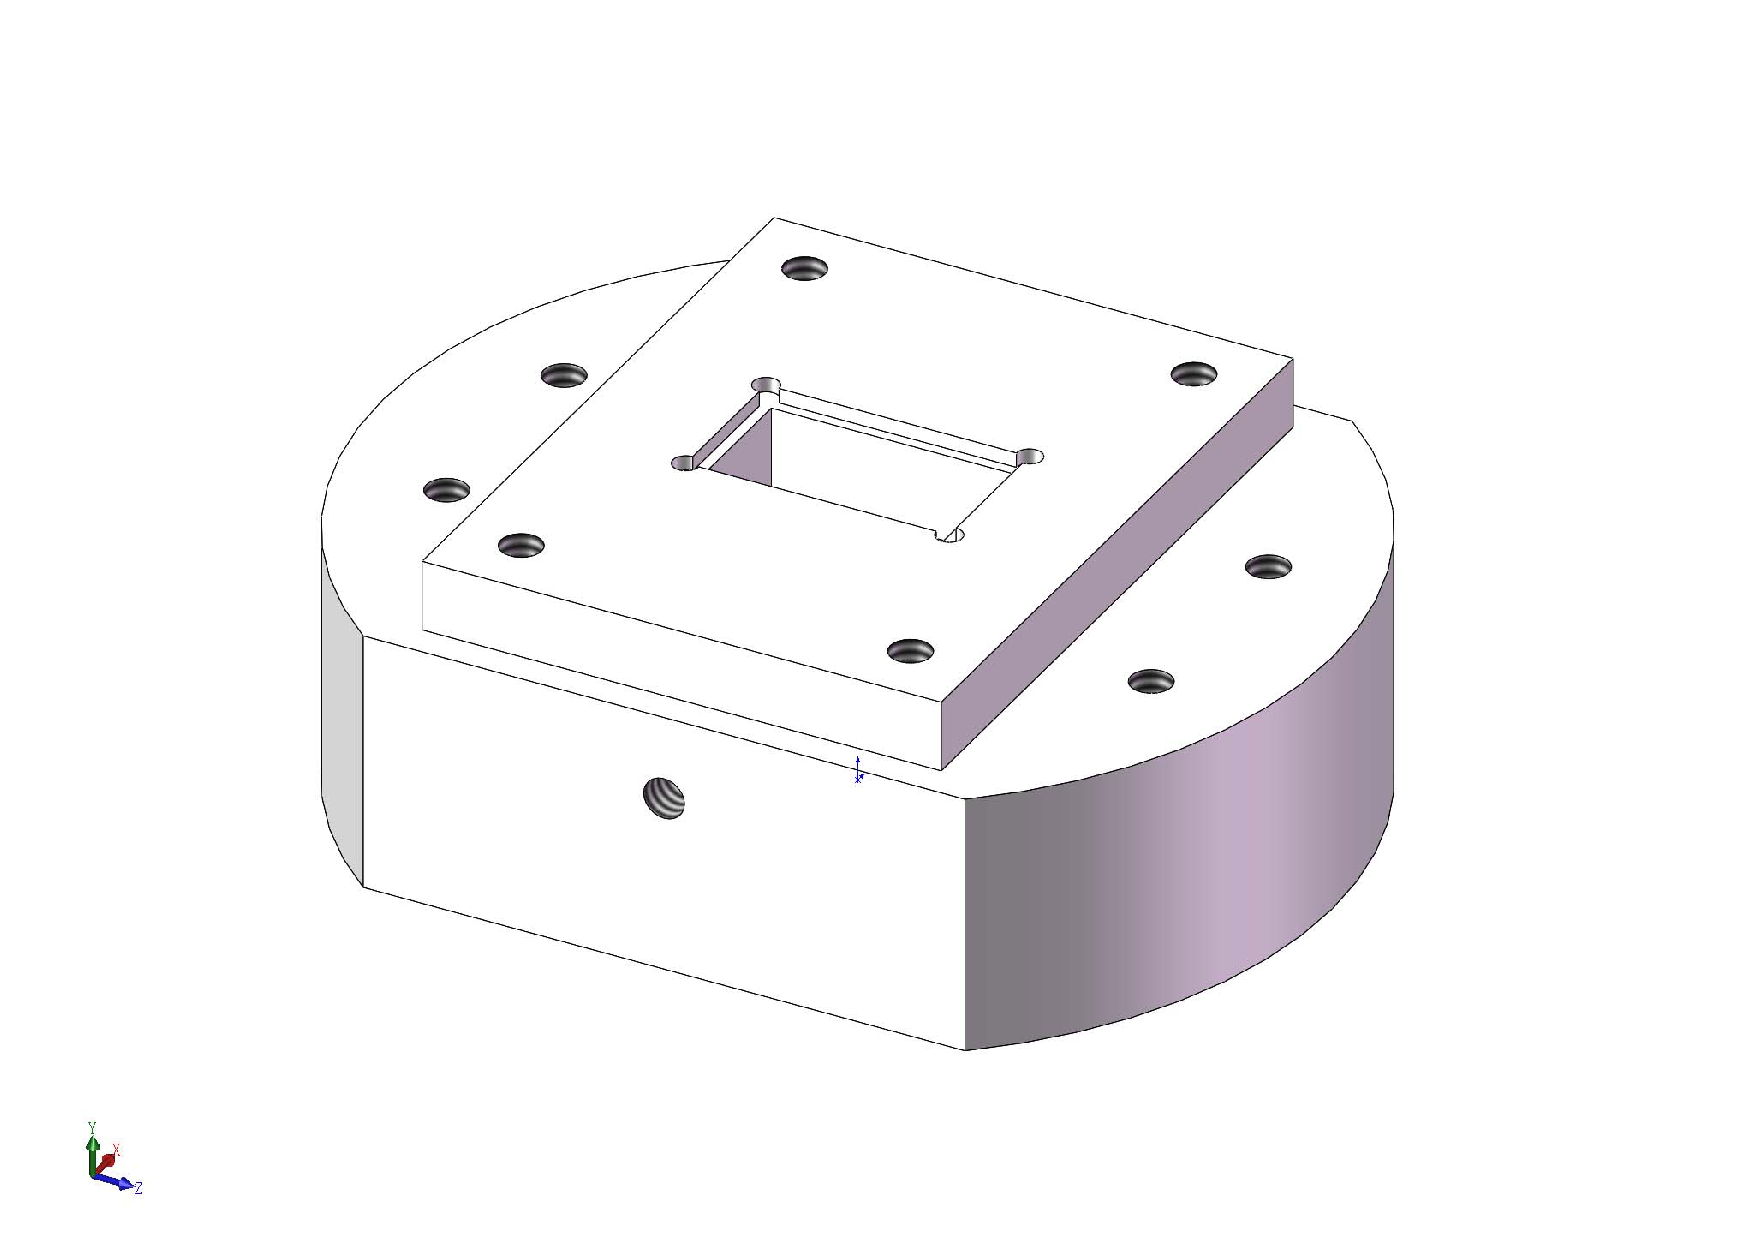
\includegraphics[width=2.2in,angle=270]{Smallbox2.pdf}
    % \caption{第二个小图形,注意这个图略矮些。subfigure中同一行的子图在顶端对齐。}
  \end{subfigure}
  \caption{原有样品盒盖子与底座设计}
  \label{fig:oldSampleBox}
\end{figure}
                  












\begin{figure}[h]
  \centering%
  \begin{subfigure}{0.4\textwidth}
    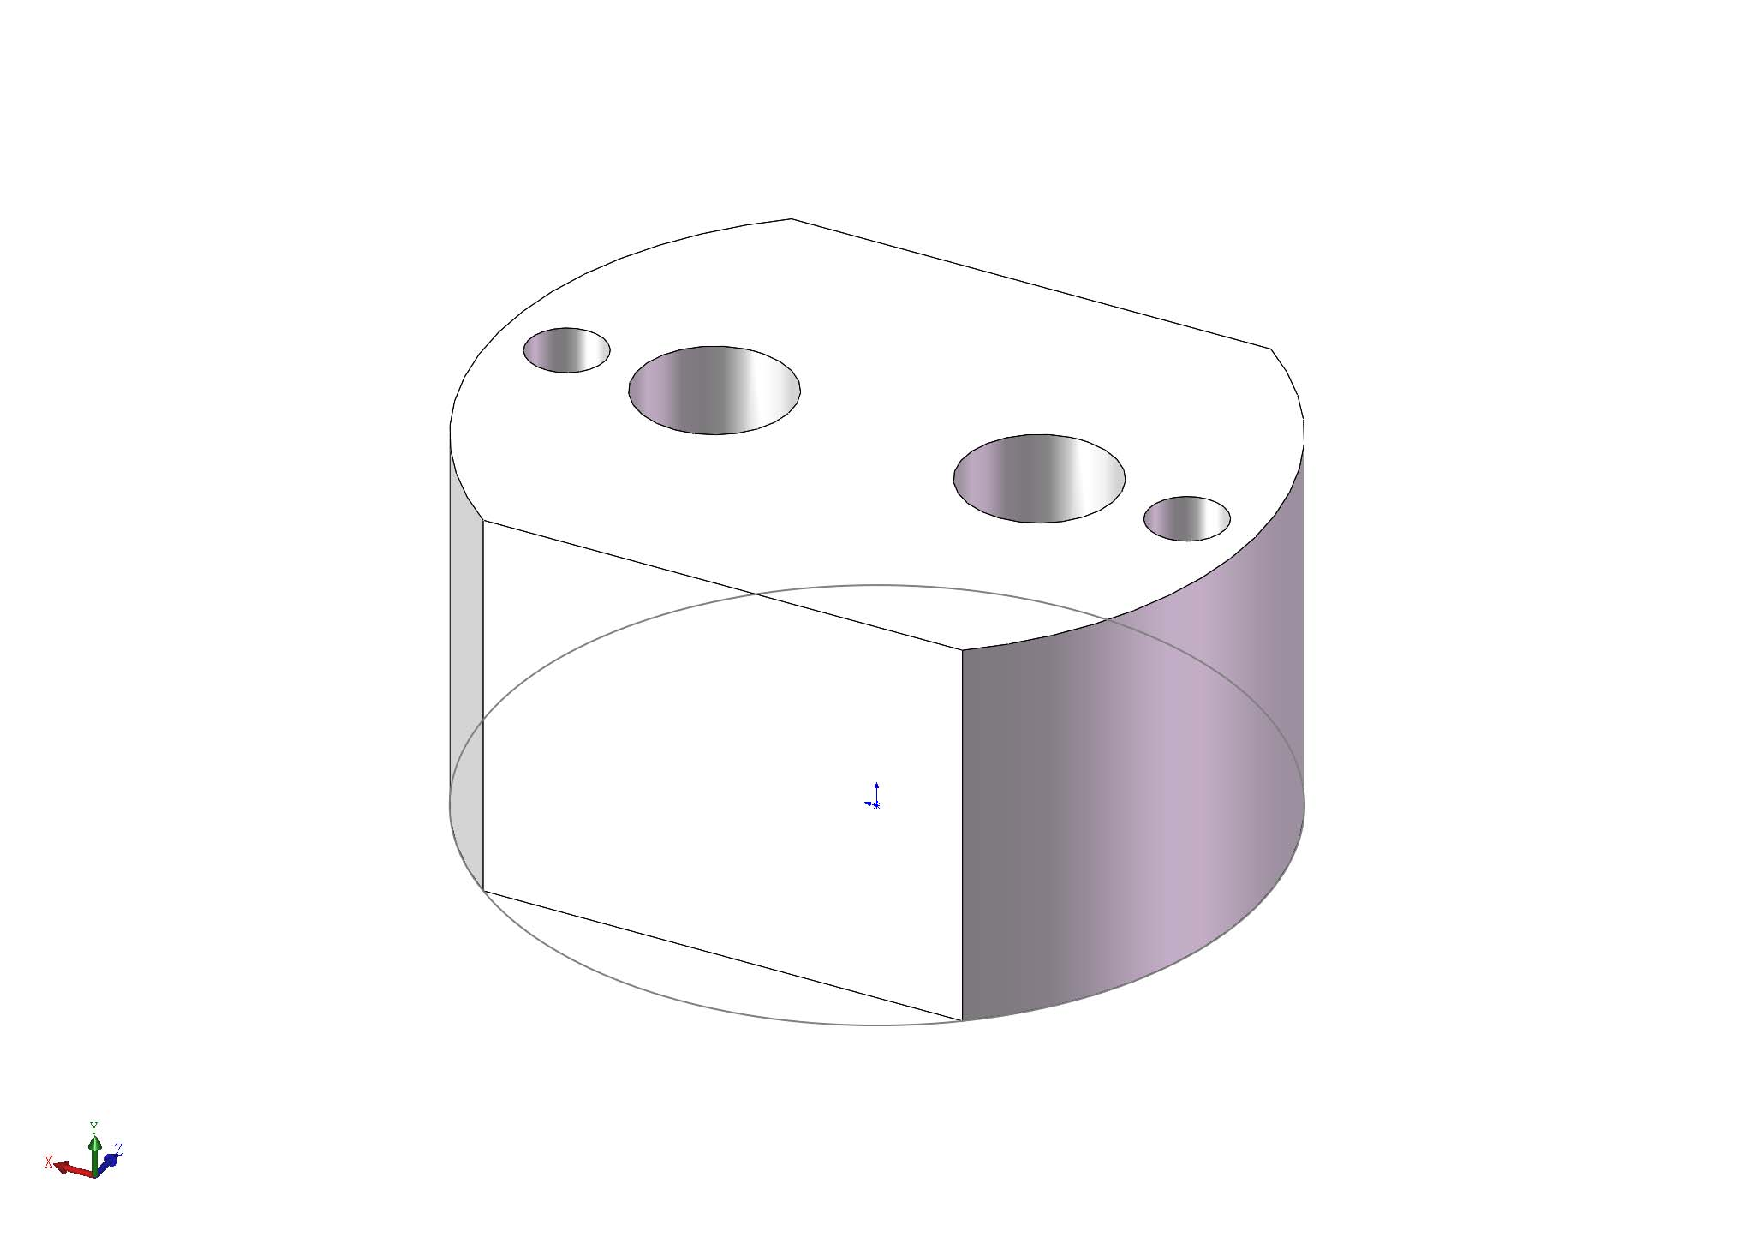
\includegraphics[width=2.2in,angle=270]{SmallboxCover.pdf}
    % \caption{第一个小图形}
  \end{subfigure}%
  % \hspace{4em}%
  \hfill
  \begin{subfigure}{0.4\textwidth}
    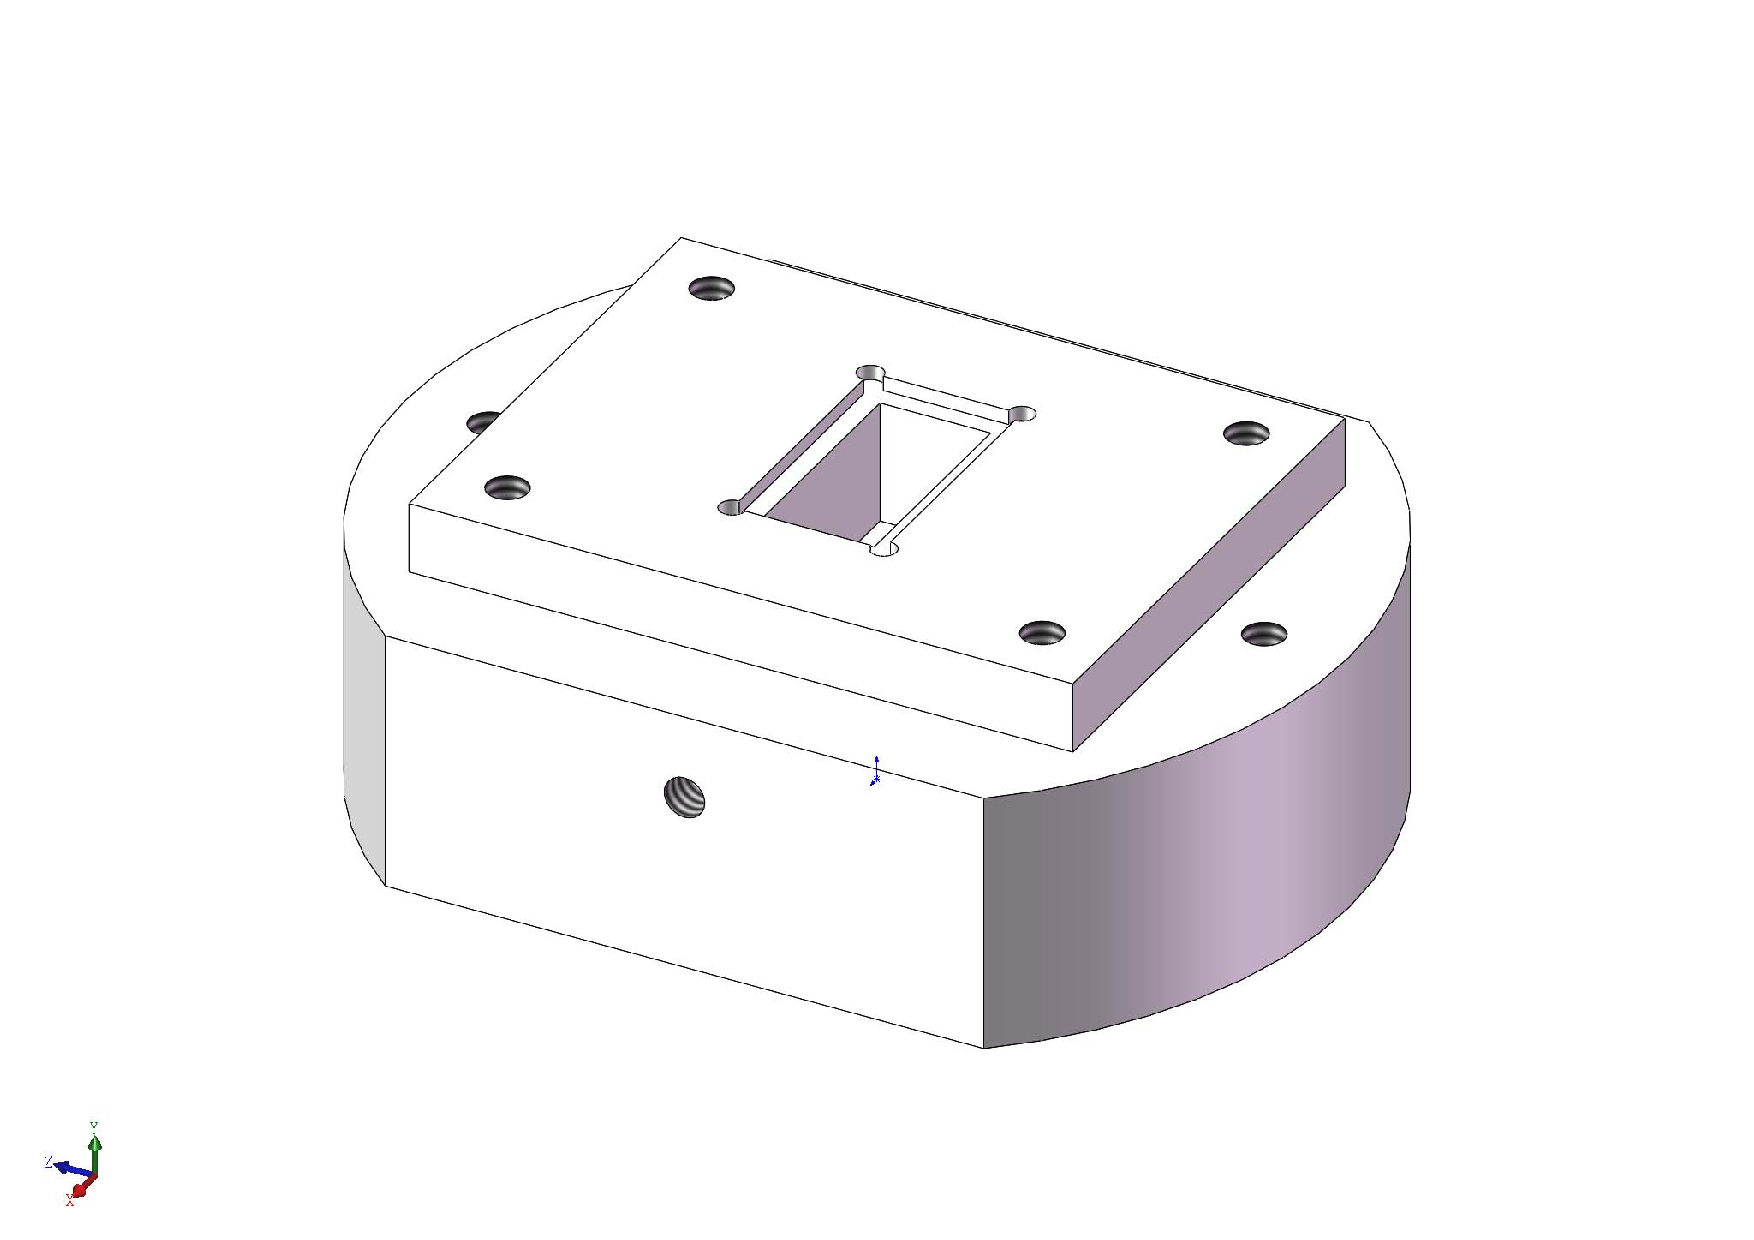
\includegraphics[width=2.2in,angle=270]{SmallboxHolderHori.pdf}
    % \caption{第二个小图形,注意这个图略矮些。subfigure中同一行的子图在顶端对齐。}
  \end{subfigure}
  \caption{改进后样品盒盖子与底座设计}
  \label{fig:newSampleBox}
\end{figure}











\begin{figure}[h]
  \centering%
  \begin{subfigure}{0.4\textwidth}
    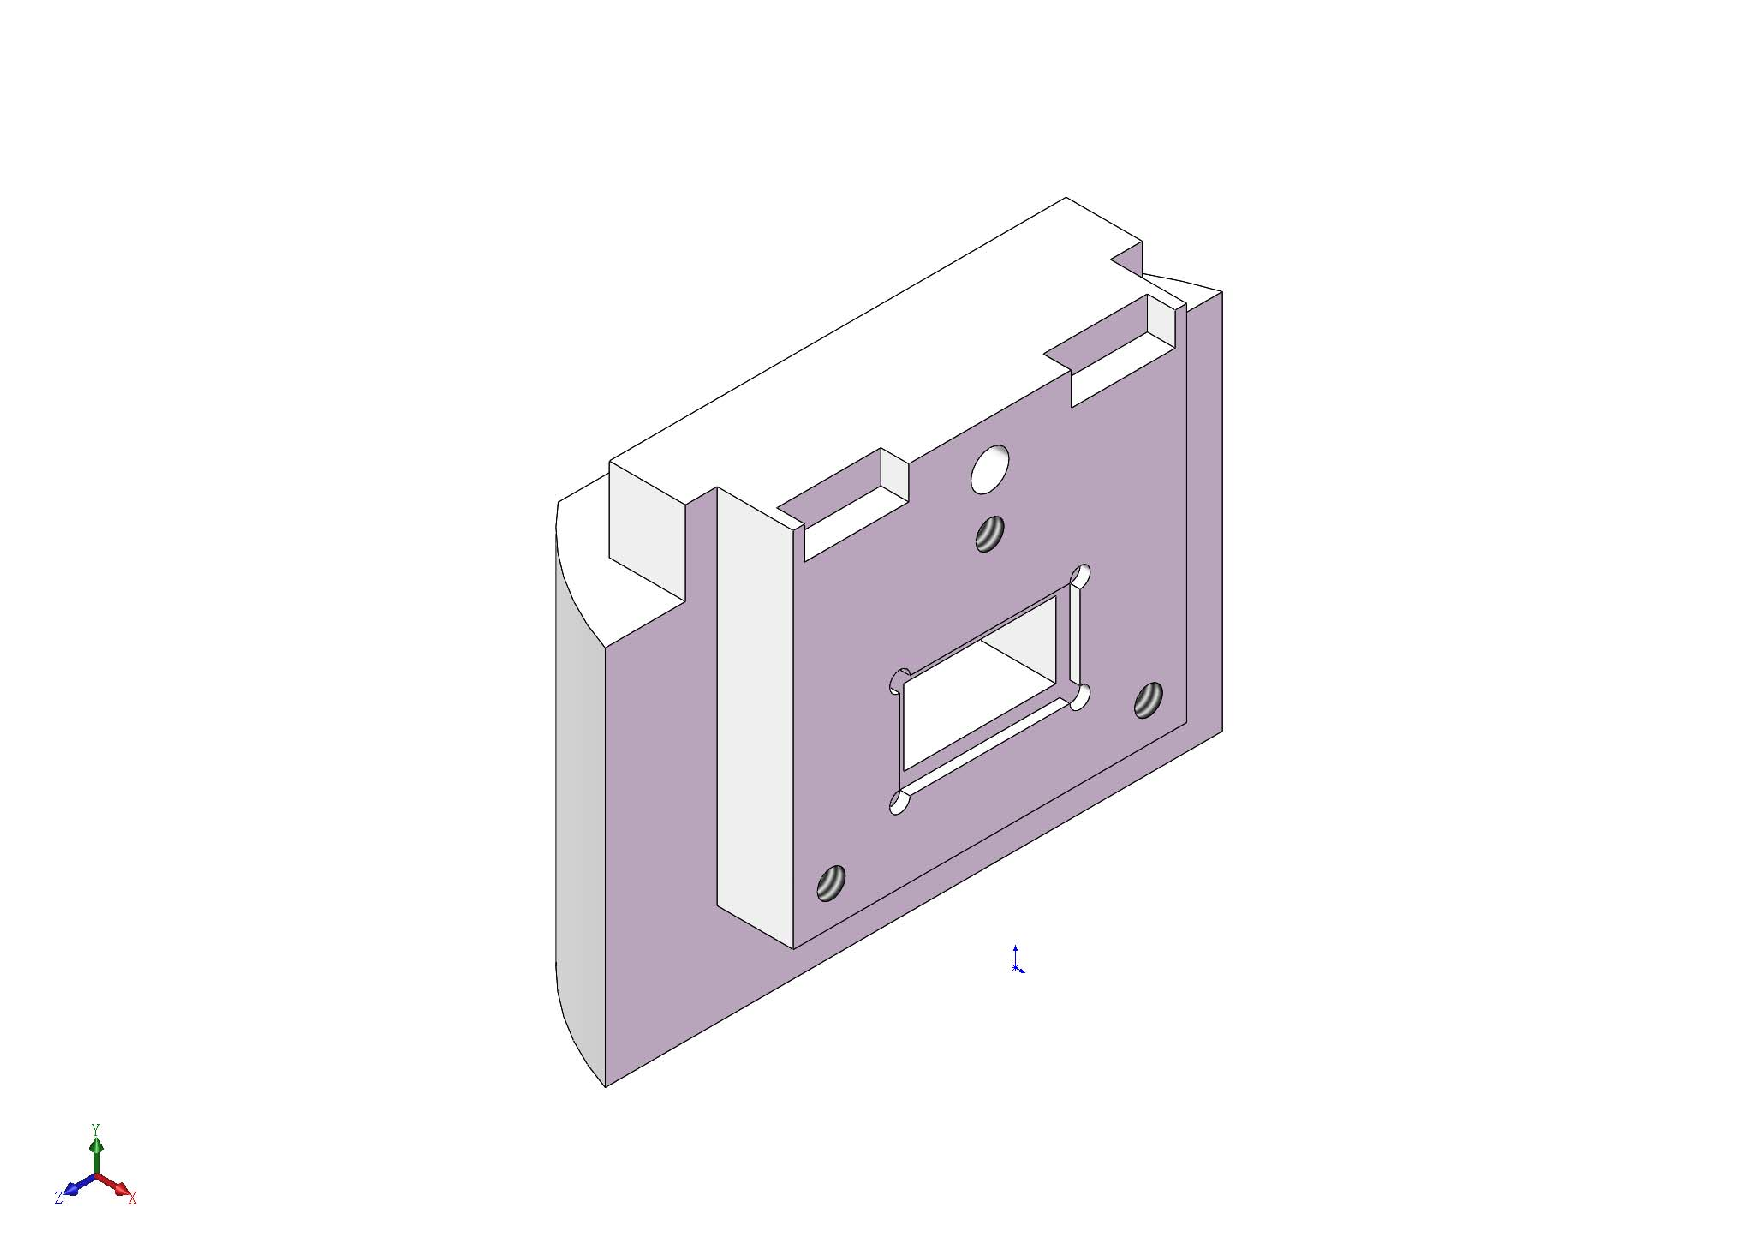
\includegraphics[width=2.2in,angle=270]{SmallboxHolderVertTotalHolder.pdf}
    % \caption{第一个小图形}
  \end{subfigure}%
  % \hspace{4em}%
  \hfill
  \begin{subfigure}{0.4\textwidth}
    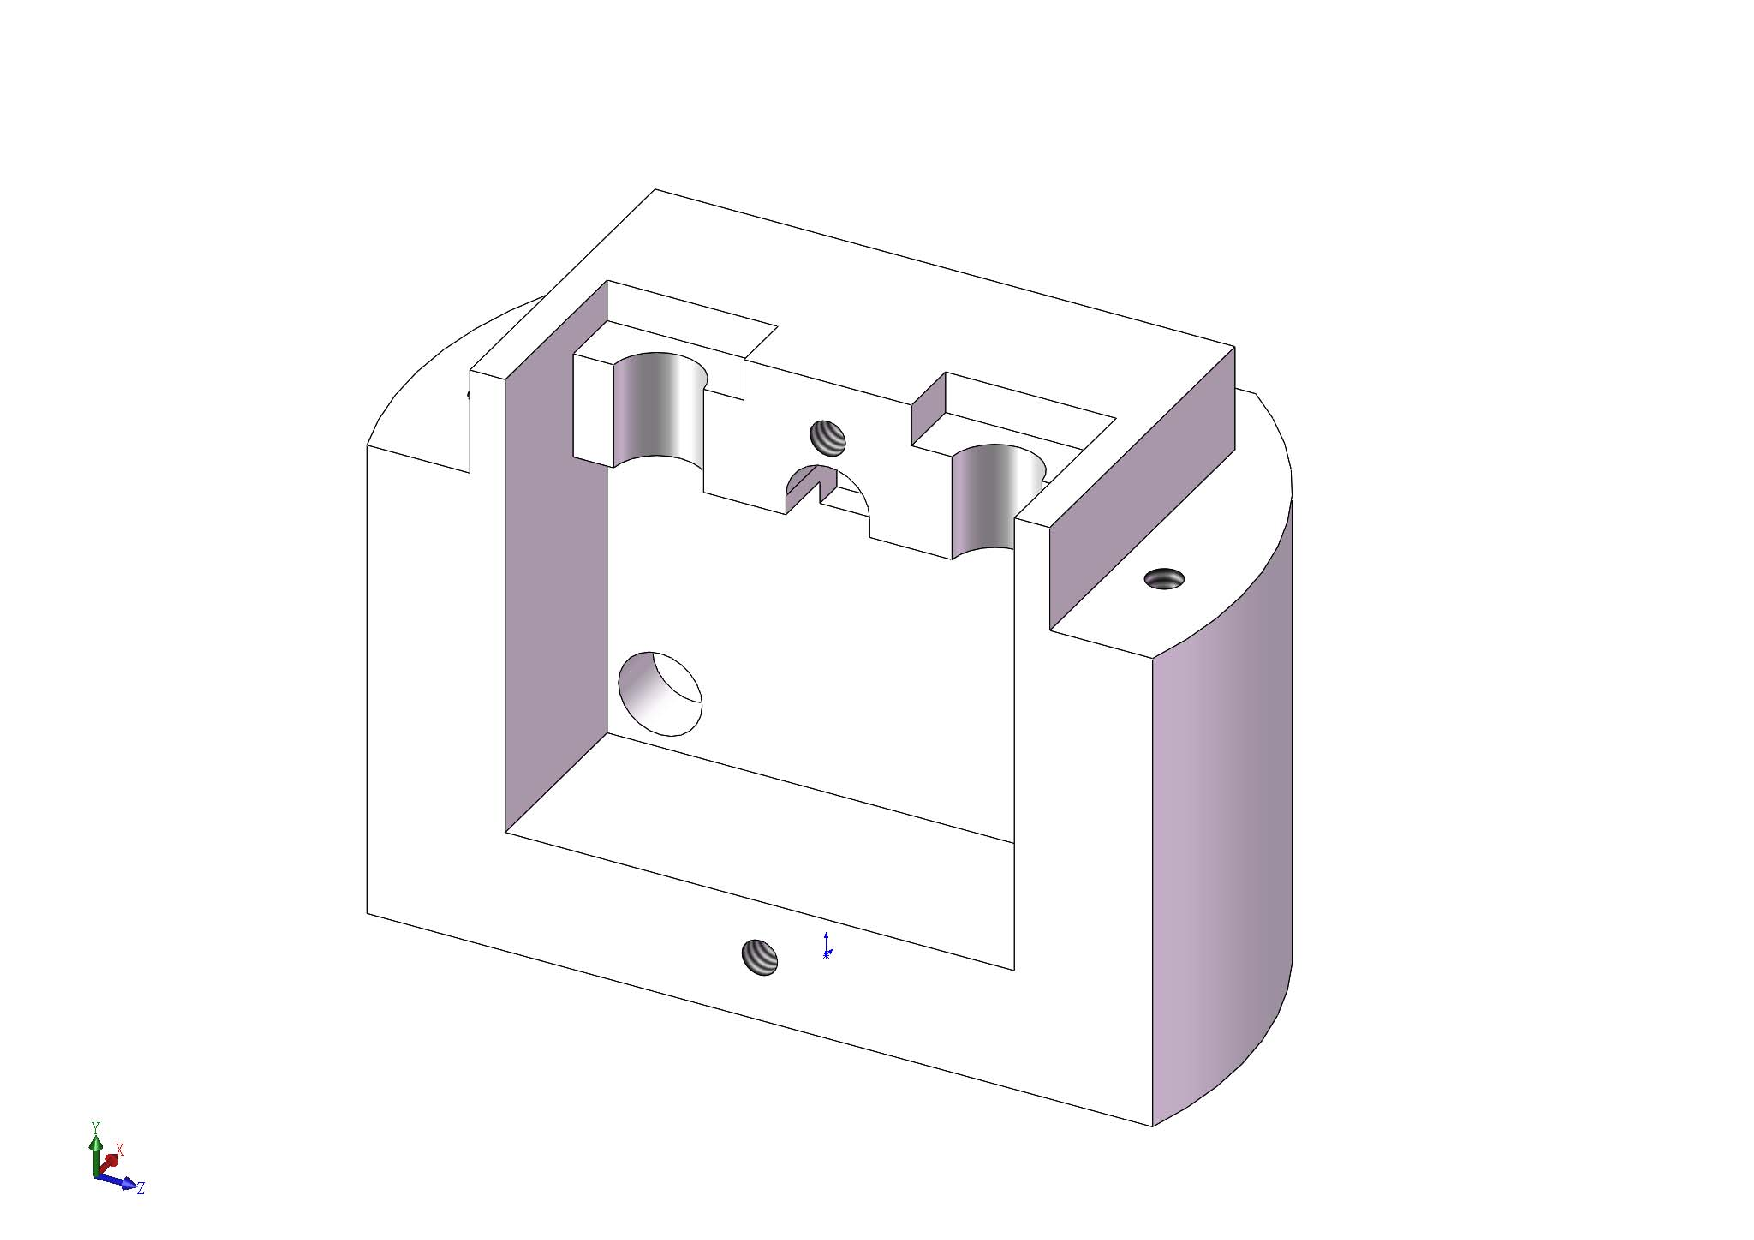
\includegraphics[width=2.2in,angle=270]{SmallboxHolderVertTotalCover.pdf}
    % \caption{第二个小图形,注意这个图略矮些。subfigure中同一行的子图在顶端对齐。}
  \end{subfigure}
  \caption{为竖直放样品所所设计的样品盒底座拆分出的盖子与底座设计}
  \label{fig:newVertiSampleBox}
\end{figure}

                  


\begin{figure}[h]
  \centering%
  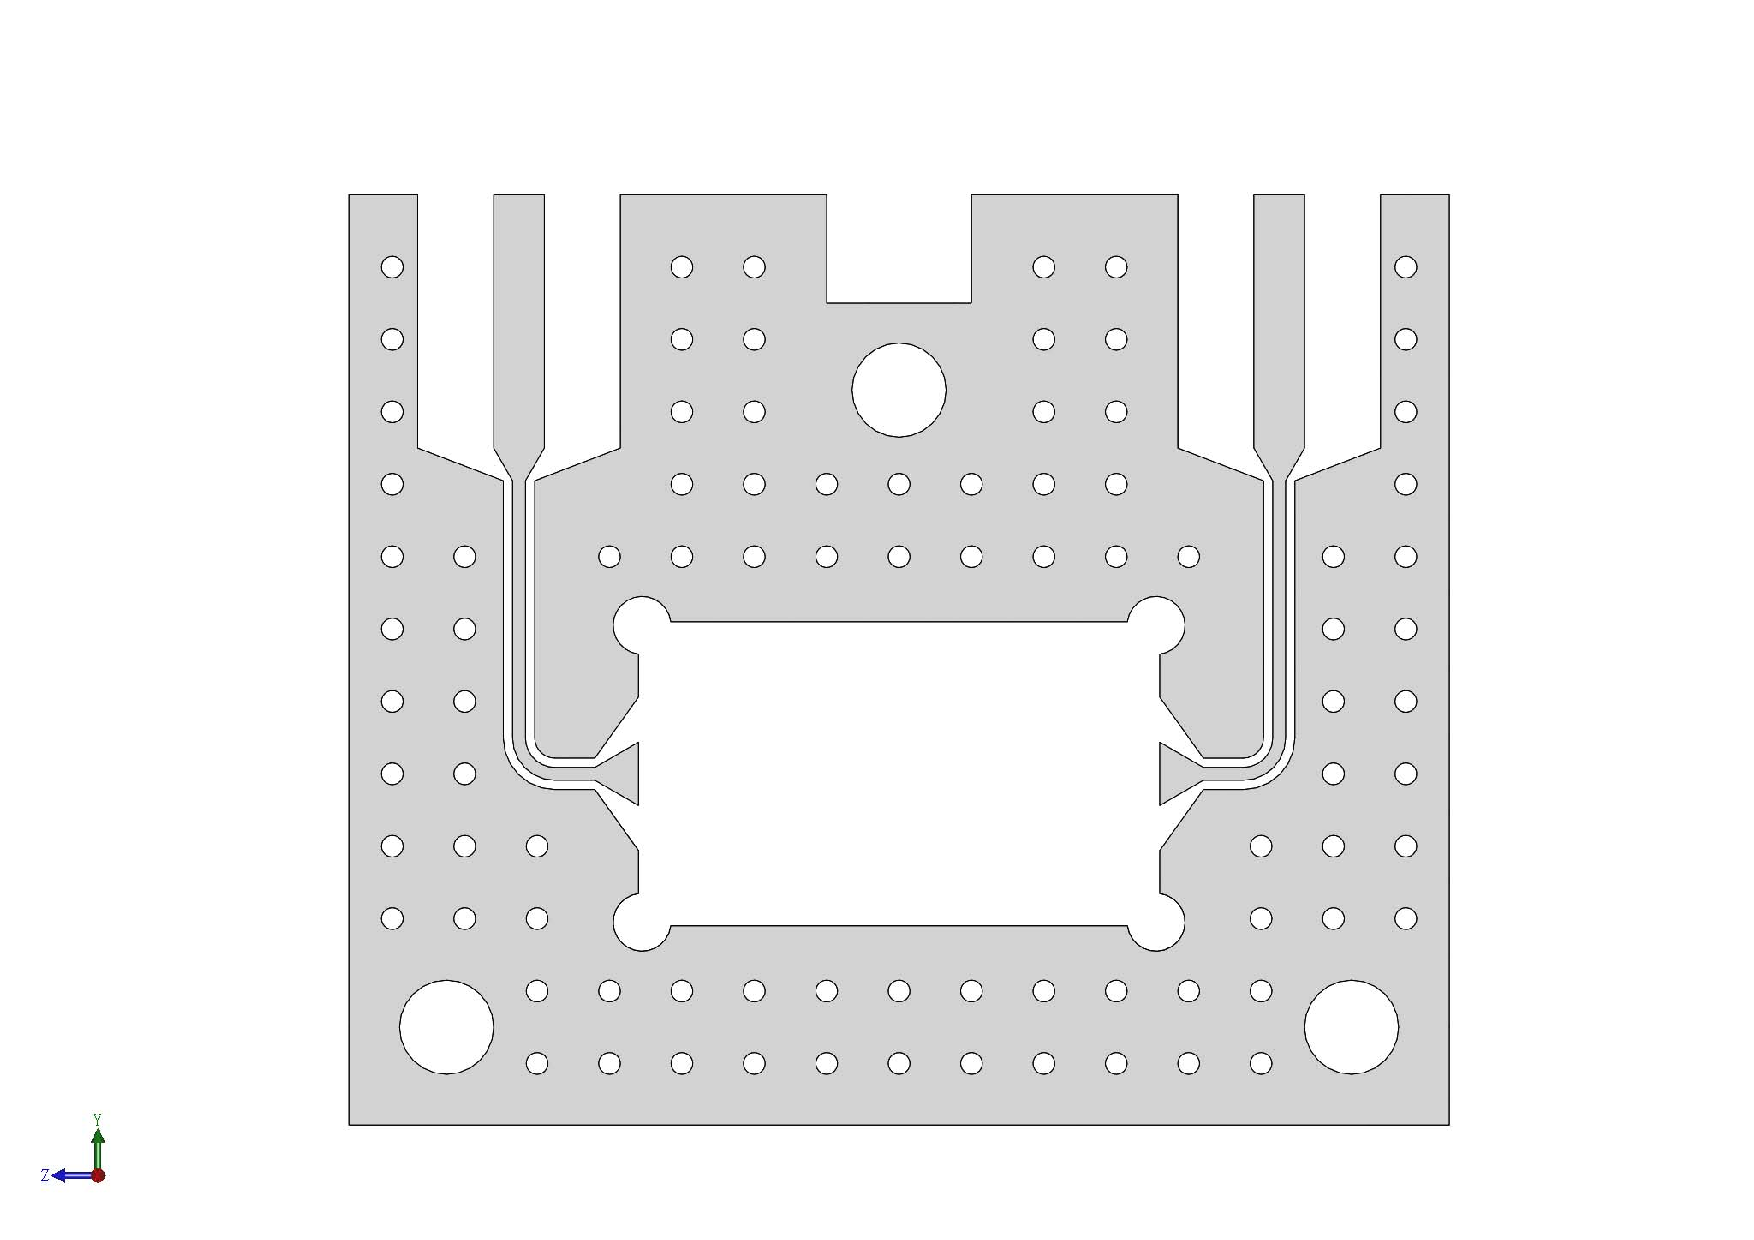
\includegraphics[width=5in,angle=270]{SmallboxHolderVertTotalHolderPCBV2.pdf}
  \caption{为新的竖直放置样品的样品盒所设计的PCB板}
  \label{fig:SmallboxHolderVertTotalHolderPCBV2}
\end{figure}






            % subsection 样品托的设计与优化 (end)



%!TEX root = ../main.tex
\chapter{2.5维谐振腔的制备与测量} % (fold)
\label{cha:2_5维谐振腔的制备与测量}
	


        \section{器件测量与制备工艺概述} % (fold)
        \label{sec:制备工艺概述}

            由于2.5维谐振腔的电容部分由上下两层金属以及中间的介电层组成,工艺较为复杂,需要至少三步光刻来完成。而细小的电感部分则需要电子束曝光(EBL)来定义形状,再由蒸发镀膜完成。因此,总的制备工艺大致如下:

            \begin{enumerate}
                \item 通过光刻,磁控溅射蒸镀金属Nb,Lift off三步制作平面波导与三层电容的第一层
                \item 通过ALD生长Al$_2$O$_3$,或通过PECVD生长SiO$_2$或SiN$_x$作为三层电容的介电层
                \item 光刻定义掩膜后通过ICP刻蚀或湿法刻蚀介电层
                    \begin{enumerate}
                        \item 剩余的介电层仅遮盖住三层电容的底层
                    \end{enumerate}
                \item 利用光刻制作出三层电容的顶层图案并蒸镀金属,对准精度约1微米,Lift off
                \item 利用EBL制作微小电感图案
                    \begin{enumerate}
                        \item 电感图案将与三层电容的上下级板相连
                        \item 对准精度 100-1000 nm
                    \end{enumerate}
            \end{enumerate}


            每一步制备工艺的具体步骤与相关参数均在附录\ref{cha:fabrication}中给出。
            
        % subsection 制备工艺概述 (end)

        \section{光刻板的设计与改进} % (fold)
        \label{sec:光刻板的设计}

            由于制备工艺需要三步光刻,对于完整制备一个器件来说,需要的光刻板的图案为一组三个,分别对应\ref{sec:制备工艺概述}制备工艺概述中的前三步。第一步完成二维平面波导以及接地平面的制作,以及三维电容的第一层金属。第二步在生长介电材料后通过光刻制作掩膜覆盖住需要保留的电容的第二层介电层部分,并刻蚀掉没有被覆盖掉的电介质。第三部制作出电容最上层的金属。最后一步通过电子束曝光与蒸镀制作微小的电感部分,并各自与三维电容的上、下两层连接起来。光刻的三个步骤所需的模板作图如图所示
            

            \begin{figure}[h]
                \centering
                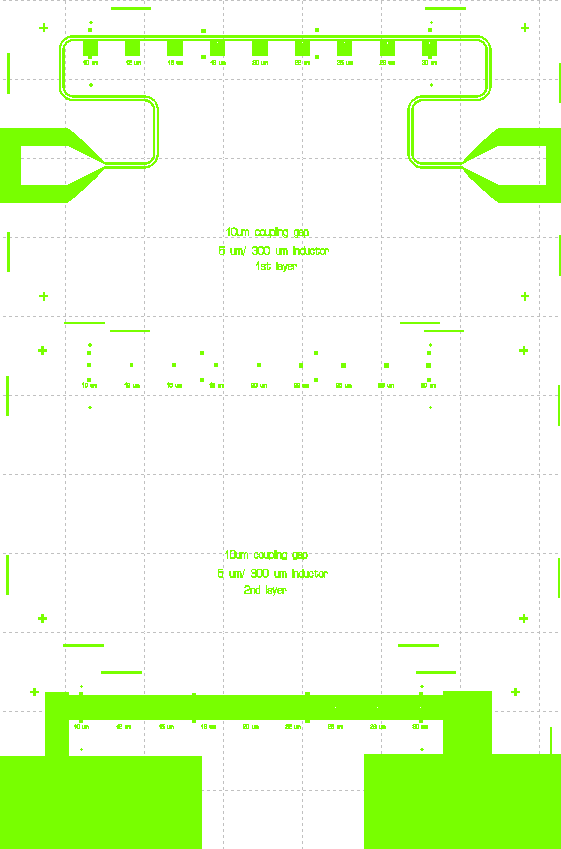
\includegraphics[width=3in]{one_group.png}
                \caption{制备一个器件所需的三个光刻步骤对应的一组三个模板图案}
                \label{fig:one_group}
            \end{figure}

            \begin{figure}[h]
                \centering
                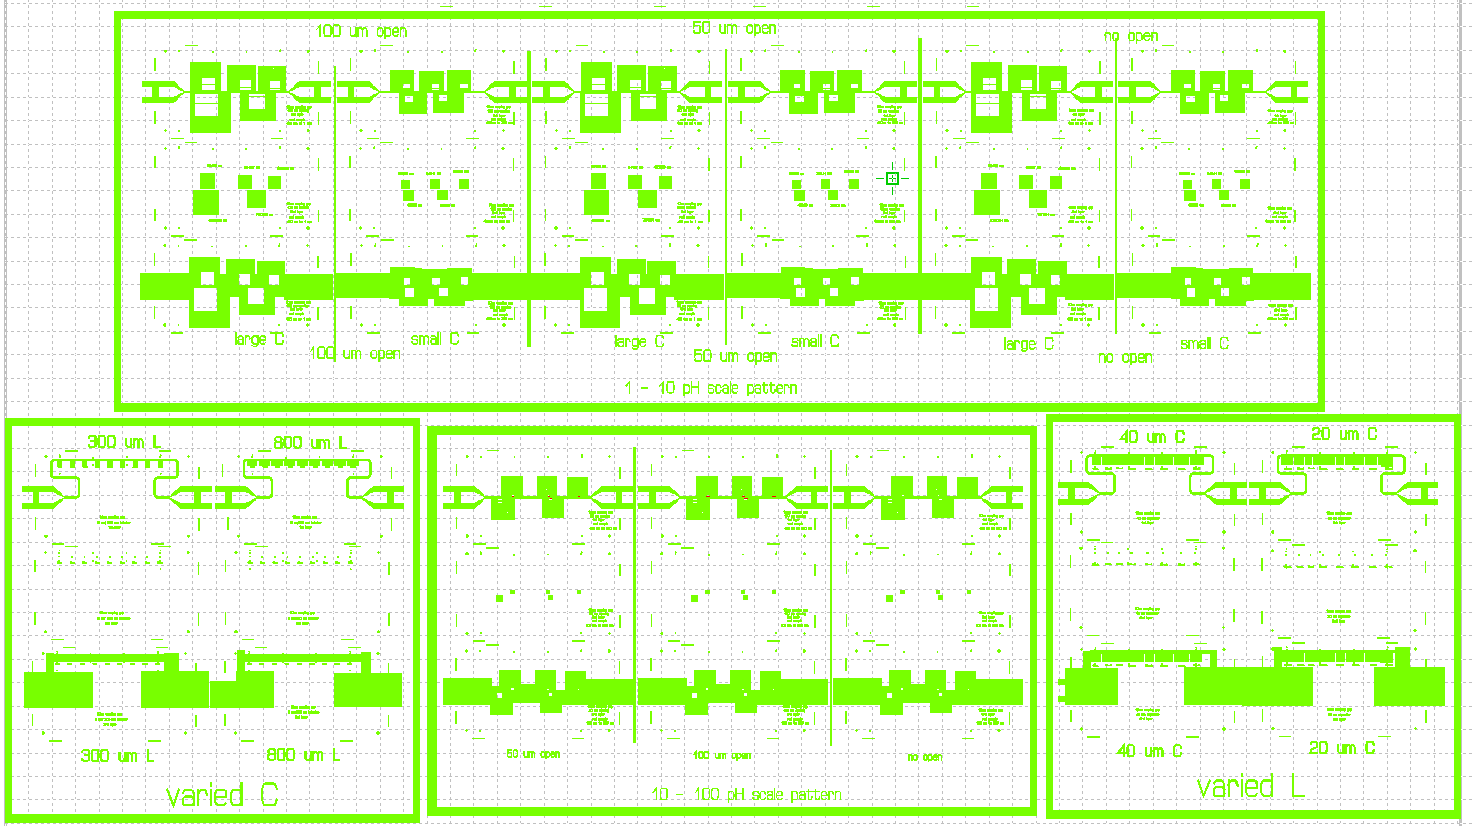
\includegraphics[width=5in]{LC.png}
                \caption{完整的光刻板图案}{}
                \label{fig:LC}
            \end{figure}

            由于没有这类谐振腔的制备经验,对于其频率的估算并没有太多把握,因此我们希望有尽可能多的谐振频率与设计相对应的数据,来辅助下一步对仿真结果的修正与器件制备的改进。由于对电容和电感估值的准确度均有待确认,我们需要至少两组不同的器件设计的组合,一组固定$L$变化$C$的大小,另一组固定$C$变化$L$的大小,这样可以通过拟合确定出每个器件的$L$与$C$的值。因此,一个二维平面波导可以与多个谐振腔耦合,可方便测量。另一方面,考虑到电子束曝光难度与耗时均较大,我们打算先尝试中等数值的电容与电感组合,使电感的尺寸能够通过光刻制备,这样即可在三层电容制备的最后一步同时制作出电感,省去了电子束曝光制备电感的步骤,大大加快样品制备与测试速度。解决三层电容的制备后,再通过电子束曝光制作电感。

            综合上述讨论,我们总共设计了若干种不同的模板几何形状,如图\ref{fig:LC}所示,覆盖了较大范围的电容与电感值,为第一次摸索器件制备工艺以及尝试性测量提供较大的频率变化区间,尽可能保证能够测到谐振腔的共振频率。


            \section{器件制备情况与讨论} % (fold)
            \label{sec:器件制备情况与讨论}
                按照上述计划,我进行了器件制备的工作,目前已完成了完整的器件制备流程。

                
            % section 器件制备 (end)
            



            \section{谐振腔响应信号的拟合} % (fold)
            \label{sec:谐振腔响应信号的拟合}
            	












\nocite{*}

%%% 其它部分
\backmatter

%% 本科生要这几个索引,研究生不要。选择性留下。
% 插图索引
\listoffigures
% 表格索引
\listoftables
% 公式索引
\listofequations


%% 参考文献
% 注意:至少需要引用一篇参考文献,否则下面两行可能引起编译错误。
% 如果不需要参考文献,请将下面两行删除或注释掉。
\bibliographystyle{thuthesis}
\bibliography{ref/refs}


%% 致谢
%!TEX root = ../main.tex

% 如果使用声明扫描页,将可选参数指定为扫描后的 PDF 文件名,例如:
% \begin{ack}[scan-statement.pdf]
\begin{acknowledgement}
  感谢两年前段路明教授容许我加入他麾下的实验室学习与工作,让我接触到了许多珍贵的科研资源并学到了众多难得的知识与技能。没有这个环境,我的学习与科研能力将比现在不知低到哪里去。感谢宋祎璞副研究员在这两年期间以及毕设期间对我的耐心指导与支持,使我从做人做事做科研等很多方面都获益匪浅。感谢卢芳超学姐,薛潇学长在我刚进组一无所知时的耐心解说与指导。感谢张宏毅学长在毕设期间在器件制备和其他诸多方面给予我的众多帮助,讨论与悉心指导,否则我不可能完成实际器件的制备。感谢郭星翰同学对PPMS系统的硬件改造以及与我时常进行的讨论。感谢熊昊楠同学对PPMS系统的使用与反馈,与你一直以来时常进行的讨论让我学习了很多。感谢孙麓岩老师及其研究组,在你们实验室借过不少东西,参观与学习了很多,与你们的讨论总是让我开阔眼界,有所收获。感谢马玉林学长对我使用切片机的帮助,以及时常借我门卡。感谢超净间的所有工作人员,没有你们的工作根本不可能有器件制备所需的众多条件。

  在2016年暑期于斯坦福的两个月暑期研修,承蒙Amir Safavi-Naeini助理教授与Rishi Patel学长的指导,让我更加熟悉MATLAB的使用与仪器的编程控制。

  感谢物理系学堂班在许多方面提供的支持,感谢朱邦芬老师与李师群老师对学堂班学生的发展的关心与支持。感谢物理系的领导与行政人员,在很多我不知道的地方为我提供了很多服务。感谢物理系的众多老师与课程让我从几乎一无所知变得似乎不那么一无所知。感谢物理系两位辅导员的辛勤工作。感谢物理系的众多同学时常与我分享他们的知识与想法,让我从他们身上学会了很多。感谢计算机辅修,让我接触与领会程序员尽量不做重复的事情的哲学以及增强了我的编程能力。

  感谢我的父母和亲人为我设定的初始参数,成长环境和后勤保障。这三个词虽然简单,但都无比重要,也让我时刻感到侥幸。

  感谢听涛食堂西侧窗口的早餐师傅在这学期的每天早上都在擀肉夹馍的面饼的间隙中微笑着满足我在龙须臊子面里加馄饨里才会有的紫菜的无理要求,让我每天都能在感受别人的善意之中开始。感谢蒙民伟科技楼的后勤人员时常帮我签收快递。感谢 \thuthesis,它的存在让我的论文写作轻松自在了许多,让我的论文格式规整漂亮了许多。感谢Sublime与LaTeXTools,它们让我的写作十分舒畅。感谢其他一些不存在的东西,让我能够更加专注。

\end{acknowledgement}


%% 附录
\begin{appendix}
%!TEX root = ../main.tex

\chapter{超导量子比特的原理} % (fold)
\label{cha:SCQubitPrinciple}
  
% chapter SCQubitPrinciple (end)













\chapter{微纳加工工艺} % (fold)
\label{cha:fabrication}

\section{光刻} % (fold)
\label{sec:光刻}
    \begin{enumerate}
        \item Spin coating S1805, 500 nm
        \begin{enumerate}
            \item 500rpm, 10s, 100rpm/s
            \item 4000rpm, 45s, 2000rpm/s
            \item 0rpm, 5s, 2000rpm/s
        \end{enumerate}
        \item Bake at 115 degree C for 1 min
        \item Align mask
        \item Expose with 405 nm UV light for 9.5s, power 350W
        \item Develop in MF-319 for 45s
        \item Clean in DI-water for 1min and blow dry
    \end{enumerate}
% section 光刻 (end)

\section{介电层生长与刻蚀} % (fold)
\label{sec:介电层生长与刻蚀}
    \begin{enumerate}
        \item PECVD生长SiO$_2$速率:70nm/min
        \item PECVD生长SiN$_x$速率:16nm/min
        \item ALD生长Al$_2$O$_3$速率:
        \item MF-319刻蚀Al$_2$O$_3$速率:
        \item MF-319刻蚀光刻胶速率:
        \item ICP刻蚀SiO$_2$速率:43.3nm/min
        \item ICP刻蚀SiN$_x$速率:50nm/min
    \end{enumerate}
    \subsection{刻蚀介电层后去除光刻胶} % (fold)
    \label{sub:刻蚀介电层后去除光刻胶}
        \begin{enumerate}
            \item 置于PG Remover中加热至85摄氏度,将烧杯口用铝箔纸盖住,保持85度30分钟
            \item 用丙酮,IPA清洗,氮气枪吹干
        \end{enumerate}
    % subsection 刻蚀介电层后的lift_off (end)
% section 介电层生长 (end)

\section{光刻胶Lift off} % (fold)
\label{sec:光刻胶lift_off}
        \begin{enumerate}
            \item 于NMP去胶液或丙酮中浸泡一晚,用铝箔纸盖住烧杯口
            \item 加热至85摄氏度15至30分钟,用铝箔纸盖住烧杯口
            \item 用镊子夹住片子后用胶头滴管于去胶液中吹洗
            \item 对于难以去除的区域,可尝试超声
            \item 对于生长了介电层后的器件,超声时应小心勿将介电层超声至脱落。对于30nm的SiO$_2$或30nm的SiN$_x$,可用60\% 功率,45kHz超声10秒,重复三次,即可去除对2.5维谐振腔样品可能出现的lift off不完全的情况,并保证介电层完整
            \item 目前尝试过用100\%功率,45kHz超声15秒,仍可保证介电层完整
            \item 从去胶液中取出后迅速放入丙酮中清洗,随后再放入IPA中清洗,最后用氮气枪吹干
        \end{enumerate}
    % section lift_off (end)

\section{磁控溅射镀膜} % (fold)
\label{sec:磁控溅射镀膜}
    \begin{enumerate}        
        \item Transfer to sputter chamber
        \item chamber -> Process
        \item open Ar valve, 100 sccm
        \item set DC parameter, I = 100mA
        \item DC -> on. If error, try with shutter open
        \item set I = 400mA
        \item set Ar to 6sccm
        \item set chrono end action to DC \& RF off and sputter shutters off
        \item Holder motion: Rotate
        \item open shutter and timing with chrono
        \item 25nm/min for sputtering Nb, hence 4min total time for 100nm Nb
        \item wait until end
        \item set Ar to 0sccm, close Ar valve
        \item Stop rotation, Chamber -> pump
        \item Holder motion -> transfer, start
        \item Transfer after pressure stable and chip cool
    \end{enumerate}
% section 磁控溅射镀膜 (end)

\section{Argon milling去除氧化层} % (fold)
\label{sec:argon_milling去除氧化层}


\begin{enumerate}
    \item transfer to oxid chamber
    \item Process-> IonGun
    \item Holder motion -> Target -> IonGun, start. Might error, start again
    \item Open Ar valve, set to 6sccm
    \item set Vbeam = 250V, Ibeam = 10mA, Vacc = 60V. Input parameters again even if they are already correct
    \item Discharge on, wait stable
    \item Beam on, wait 2min
    \item set Vbeam = 400V, Ibeam = 20mA, Discharge 40V, Vacc = 60V, Iacc = 1.1mA, wait stable
    \item ordinary status: pressure 1.2e-4Torr, cathode 7.1V, 6.22A, 40V/0.23A, 399V/20.1mA, 60V/1.1mA
    \item Set chrono end action to IonGun off
    \item open shutter and timing with chrono, 3min30s
    \item wait until end
    \item close shutter
    \item Ar off, Ar valve off
    \item oxid chamber -> pump
    \item Holder motions -> Transfer, start
    \item transfer after pressure stable
\end{enumerate}

% section argon_milling去除氧化层 (end)

\section{点焊} % (fold)
\label{sec:点焊}
    \begin{enumerate}
        \item 一焊由于PCB上的SMP接头的空间位置原因需位于器件上,二焊位于PCB板上,焊接使用铝线
        \item 一焊参数:功率220,时间30ms,力19
        \item 二焊参数:功率330,时间40ms,力19
        \item 点焊时应使焊线尽可能地短而密
    \end{enumerate}
% section 点焊 (end)
  

















% chapter fabrication (end)

\chapter{PPMS系统的常用操作} % (fold)
\label{cha:ppms系统的常用操作}
    对于PPMS的详细介绍可参阅PPMS的用户手册,本附录在读者熟悉PPMS相关术语与参数(如Chamber Pressure等)的前提下,为使用者提供一个方便参考的操作流程。

    在正常的测量状态下,Chamber Pressure与样品室温度有关,样品温度为2K左右时一般为300至400mTorr,chamber state应该为Purged,意为样品室已用He气清洗并抽真空。在非远程控制PPMS时,一般通过与PPMS相连的电脑上的MultiVu程序控制PPMS。该程序主面板下方有若干小面板,点击这些小面板可调出设定温度,磁场与样品室状态的分面板。常用的分面板也即前文提到的Temperature,Chamber,Field面板。

    \section{调节温度与磁场} % (fold)
    \label{sec:调节温度}
        在Temperature面板中,status显示当前样品温度。通过Control一栏即可设置目标温度(set point)以及调温的速率(Rate)。Mode选项有Fast settle和No overshoot两种,也即快速和非振荡的平稳到达目标温度两种模式。

        升温时最大速率不应超过20K/min,降温时最大速率不应超过10K/min。


        调节磁场与调节温度十分类似。
    % section 调节温度 (end)

    \section{更换样品} % (fold)
    \label{sec:更换样品}
        首先升温至室温,300K,从2K开始升温则需约30分钟。样品室升至常温后,样品室气压约为20~40Torr。点击Chamber分面板的Vent/Seal,此时样品室气压将快速升至常压,约790Torr,此后即可取出样品杆。若取出样品杆时间较长,应插入空样品杆并点击Chamber分面板的Purge/Seal以使样品室处于较好的密封环境。

        更换完样品并插入封好样品杆后,点击Chamber分面板的Purge/Seal,此时state变为Purging。样品室气压将在常压与~30Torr间来回反复若干次,约5分钟后state变为Purged,此时即可开始制冷。
    % section 更换样品 (end)
% chapter ppms系统的常用操作流程 (end)















\chapter{测量系统MATLAB代码} % (fold)
\label{cha:measurement_code}

通过MATLAB控制仪器,能够十分方便地调整仪器的各项参数以及从仪器采集所需数据。对于封装较好的代码,能够可扩展地编写与控制更为复杂的实验。因此我通过MATLAB实现了对VNA的控制与数据采集,基于PPMS仪器商提供的动态链接库文件实现了对PPMS系统的状态读取与控制。在这二者的基础上,编写了扫描不同温度与磁场下的频率响应的实验的代码。

本附录中将给出VNA与PPMS的MATLAB控制程序代码,以及扫描温度与磁场的MATLAB代码。


  \section{VNA控制代码} % (fold)
  \label{sec:vna控制代码}

  \begin{lstlisting}
classdef E5071C < handle
    % E5071C describe and control the agilent E5071C ENA
    %
    % EXAMPLES (assume instance named 'vna'):
    %   initialization:
    %       vna = E5071C;
    %       vna = E5071C('address',8,'InputBufferSize',100000);
    %   set & get parameters
    %       % fetch & return the start frequency:
    %       freq = vna.freqStart;
    %       % fetch & return the IFBW:
    %       bw = vna.ifbw;
    %       % set the stop frequency to 5GHz:
    %       vna.freqStop = 5e9;
    %       % set the number of average and turn on averaging:
    %       vna.avg = 999;
    %   fetch trace:
    %       % fetch the trace data, return a structure
    %       trace = vna.trace
    %
    %   See E5071C/plotTrace, E5071C/fit and E5071C/manualSweep for detail usage
    %
    %   Wentao, April 2017
    %
    
    properties (Constant)
        MAX_POINTS = 1601;
        MAX_AVG = 999;
        
    end

    properties
        visa
        InputBufferSize
        TimeOut
        
        address
        
        % properties with set & get methods
        freqStart
        freqStop
        freqSpan
        freqCenter        
        avg
        numOfPoints
        ifbw
        meas        
        outp
        power
        trigMode
        
        trace
        
        freqs
        h_fig       % figure handle
    end
    
    methods
        
        function obj = E5071C(varargin)
            % Initialize E5071C object
            %
            p = inputParser;
            p.addParameter('address',6, @isnumeric);        % GPIB address
            p.addParameter('InputBufferSize',30000, @isnumeric);
            p.addParameter('TimeOut',20, @isnumeric);
            p.parse(varargin{:});
            expandStructure(p.Results);
            
            obj.address = address;
            obj.TimeOut = TimeOut;
            obj.InputBufferSize = InputBufferSize;
            
            obj.visa = visa('agilent',sprintf('GPIB::%d::INSTR',obj.address));
            fprintf('%s\nConnected.\n',obj.read('*IDN?','%s'));
            set(obj.visa,'InputBufferSize', obj.InputBufferSize);
            set(obj.visa,'TimeOut', obj.TimeOut);
            % Set byte order to swapped (little-endian) format  
            fprintf('Set byte order to little-endian...');
            obj.write(':FORMAT:BORD SWAP');
            fprintf('Done.\n')
            % Set data type to real 64 bit binary block 
            fprintf('Set data type to real 64 bit binary block...');
            obj.write(':FORMAT:DATA REAL');
            fprintf('Done.\n');
        end
        
        function delete(obj)
            delete(obj.visa);
        end
        
        %% frequency set & get
        function value = get.freqStart(obj)
            value = obj.read(':sens:freq:star?', '%f');
        end
        function set.freqStart(obj,val)
            obj.write(':sens:freq:star %f',val);
        end
        function value = get.freqStop(obj)
            value = obj.read(':sens:freq:stop?', '%f');
        end
        function set.freqStop(obj,val)
            obj.write(':sens:freq:stop %f',val);
        end
        function value = get.freqCenter(obj)
            value = obj.read(':sens:freq:cent?', '%f');
        end
        function set.freqCenter(obj,val)
            obj.write(':sens:freq:cent %f',val);
        end
        function value = get.freqSpan(obj)
            value = obj.read(':sens:freq:span?','%f');
        end
        function set.freqSpan(obj,val)
            obj.write(':sens:freq:span %f', val);
        end
        
        %% sweep setup: measurement parameter, points, average, ifbw
        function value = get.meas(obj)
            value = obj.read(':CALC:PAR:DEF?', '%s');
        end
        function set.meas(obj, val)
            obj.write(':CALC:PAR:DEF %s', val);
        end
        function value = get.numOfPoints(obj)
            value = obj.read(':sens:swe:poin?', '%f');
        end
        function set.numOfPoints(obj, val)
            obj.write( ':sens:swe:poin %d', val);
        end
        
        function value = get.avg(obj)
            value = obj.read( ':sens:aver:count?', '%f');
        end
        function set.avg(obj, val)
            obj.write( ':sens:aver:count %d', val);
            obj.write(':SENSe:AVERage:STATe 1');
        end        
        function clearAvg(obj)
            obj.write(':SENSe:AVERage:CLE');
        end
        
        function value = get.ifbw(obj)
            value = obj.read(':sens:BWID:RES?', '%f');
        end
        function set.ifbw(obj, val)
            obj.write( ':sens:BWID:RES %f', val);
        end
        
        function val = sweepTime(obj)
            val = obj.read('SENS:SWE:TIME:DATA?','%f');
        end
        
        
        %% output & trigger
        function value = get.power(obj)
            value = obj.read(':SOURce:POWer:LEVel:IMMediate:AMPLitude?', '%f');
        end
        function set.power(obj, val)
            obj.write(':SOURce:POWer:LEVel:IMMediate:AMPLitude %d', val);
        end
        function value = get.outp(obj)
            value = obj.read(':OUTP:STATe?', '%f');
        end
        function set.outp(obj, val)
            obj.write(':OUTP:STATe %d', val);
        end
        function value = get.trigMode(obj)
            value = obj.read(':TRIG:SEQ:SOUR?','%s');
        end
        function set.trigMode(obj, val)
            % set.trigMode sets trigger mode
            %   available options: 'INT', 'EXT', 'MAN', 'BUS'
            %     Internal Trigger
            %     Uses the internal trigger to generate continuous triggers automatically.
            % 
            %     External Trigger
            %     Generates a trigger when the trigger signal is inputted externally via the Ext Trig connector or the handler interface.
            % 
            %     Manual Trigger
            %     Generates a trigger when the key operation of Trigger > Trigger is executed from the front panel.
            % 
            %     Bus Trigger
            %     Generates a trigger when the SCPI.IEEE4882.TRG object is executed.

            obj.write(':TRIG:SEQ:SOUR %s',val);
        end
        
        %% set & get configurations
        function setConfig(obj, config)
            % setConfig apply parameters to E5071C
            % config should have same or less fields as E5071C properties
            % with set & get methods
            flds = fieldnames(config);
            for ii = 1:length(flds)
                fld = flds{ii};
                obj.(fld) = config.(fld);
            end
        end
        
        function params = getConfig(obj)
            % getConfig returns E5071C object parameters for saving
            % configuration
            flds = {'freqStart',...
                'freqStop',...
                'freqSpan',...
                'freqCenter',...
                'avg',...
                'numOfPoints',...
                'ifbw',...
                'meas',...
                'outp',...
                'power',...
                'trigMode'};            
            for ii = 1:length(flds)
                fld = flds{ii};
                params.(fld) = obj.(fld);
            end
        end
        
        
        %% get & plot trace
        function autoScale(obj)
            % autoScale auto-scales the y axis
            % for viewing the image via web server
            obj.write(':DISP:WIND:TRAC:Y:SCAL:AUTO');
        end
        function value = get.freqs(obj)            
            value = obj.freqStart:((obj.freqStop...
                - obj.freqStart)/obj.numOfPoints):obj.freqStop;
            value = value(1:end-1);
        end
        function value = get.trace(obj)
            % adopted from https://community.keysight.com/thread/22342
            fopen(obj.visa);
            fprintf(obj.visa, 'CALC:DATA:SDAT?'); 
            [data, count, msg] = binblockread(obj.visa, 'double'); 
            fclose(obj.visa);
            value.count = count;
            value.msg = msg;
            value.X = data(1:2:end); 
            value.Y = data(2:2:end);
        end
        
        function titleStr = plotTrace(obj, varargin)
            % plotTrace fetch & plot trace data
            % EXAMPLE (assume the object is named 'vna'):
            %   vna.plotTrace;
            %   vna.plotTrace('issavefig', true);
            %   vna.plotTrace('issavefig', true,'filename','test');
            %
            % See the inputParser below for more options
            %   
            
            p = inputParser;
            p.addParameter('issavedata',false,@islogical);
            p.addParameter('issavefig',false,@islogical);
            p.addParameter('avg',1,@isnumeric);
            p.addParameter('filename','',@ischar);
            p.addParameter('format','png',@ischar);
            p.parse(varargin{:});
            expandStructure(p.Results);
            
            if avg > 1
                pause(round(avg*obj.sweepTime + 1));
            end
            
            hfig = figure;
            obj.h_fig = hfig;
            trace = obj.trace;
            
            plot(obj.freqs/1e9,...
                20*log10(abs(trace.X + 1i*trace.Y)));
            xlabel freq/GHz
            ylabel SParameter/dB
            titleStr = ['start_' num2str(obj.freqStart/1e9)...
                'GHz_stop_'  num2str(obj.freqStop/1e9)...
                'GHz_pow_' num2str(obj.power)...
                'dBm_AVG_' num2str(avg)];
            title(titleStr, 'interpreter','none');
            
            if issavefig
                if ~isempty(filename)
                    titleStr = filename;
                end
                saveas(hfig, [titleStr format]);
            end
            
            if issavedata  
                str = titleStr;
                freqs = obj.freqs;
                config = obj.getConfig;
                save([str '.mat'],'freqs','trace','str','config');
            end      
            
        end
        
        function [freqs, trace] = manualSweep(obj, varargin)
            % manualSweep defines and does a manual frequency sweep
            % main purpose is for wide sweep with high resolution for
            % finding modes
            %
            % EXAMPLE:
            %   [freqs, trace] = vna.manualSweep('start',1e9,'stop',9e9,'res',1e5);
            %   [freqs, trace] = vna.manualSweep('start',3.5e9,'stop',3.6e9,'res',1e4, 'avg',999);
            %   [freqs, trace] = vna.manualSweep('center',4.9655e9,'span',1e6,'res',0.001e6,'avg',2,'ifbw',100,'pow',-10);
            %
            %
            % See the inputParser below for more options
            %
            
            p = inputParser;
            p.addParameter('start',1e9,@isnumeric); % start frequency
            p.addParameter('stop',8e9,@isnumeric);  % stop frequency
            p.addParameter('res',1e6,@isnumeric);   % frequency resolution
            p.addParameter('avg', 1, @isnumeric);       % number of average
            p.addParameter('ifbw', 100, @isnumeric);    % ifbw of vna
            p.addParameter('points', obj.MAX_POINTS, @isnumeric); % number of points of vna
            p.addParameter('pow', -100, @isnumeric); % power of vna, default below
                                                        % the lowest power of E5071C,
                                                        % hence this
                                                        % parameter only
                                                        % takes effect if it
                                                        % is given a valid
                                                        % value
            p.addParameter('center', 0, @isnumeric);  % frequency sweep can also be defined
                                                      % by center and span,
                                                      % if they are given a
                                                      % valid value
            p.addParameter('span',0, @isnumeric);
            p.addParameter('issavedata',true,@islogical);
            p.addParameter('hfig',233,@isnumeric);      % figure handle
            p.addParameter('notes','',@ischar);         % notes to add in file name
            
            p.parse(varargin{:});
            expandStructure(p.Results);
            
            freqSectionSpan = res * points;
            freqSectionSpan = 1e6 * round(freqSectionSpan/1e6);
            if span ~= 0 && center ~= 0
                start = center - span/2;
                stop = center + span/2;
            end
            numOfSections = ceil((stop - start)/freqSectionSpan);
            stop = start + numOfSections * freqSectionSpan;
            totalPoints = points * numOfSections;
            
            % initialize
            freqs = NaN(1, totalPoints);
            trace.X = freqs;
            trace.Y = freqs;
            
            % apply parameters
            obj.ifbw = ifbw;
            if pow > -85
                obj.power = pow;
            end
            obj.numOfPoints = points;
            obj.freqSpan = freqSectionSpan;
            obj.avg = obj.MAX_AVG;
            
            sweepTime = obj.sweepTime;
            waitTime = ceil(avg * sweepTime) + 1;
            
            figure(hfig);
            xlabel freq/GHz
            ylabel SParameter/dB
            str = sprintf('start_%.2fGHz_stop_%.2fGHz_res_%.2fMHz_pow_%ddBm_AVG_%d',...
                start/1e9,stop/1e9,res/1e6,obj.power,avg);
            title(str,'interpreter','none');
            
            fprintf('\tsweep from %.2fGHz to %.2fGHz, %d sections, %ds per section\n\ttotal points: %d, total time: %ds.\n',...
                start/1e9,stop/1e9, numOfSections,waitTime,totalPoints, waitTime * numOfSections);
            for i = 1:numOfSections
                obj.freqCenter = start + freqSectionSpan/2 +  freqSectionSpan* (i-1);
                fprintf('sweeping %.2fGHz to %.2fGHz...\n',obj.freqStart/1e9,obj.freqStop/1e9);
                pause(waitTime);
                tmptrace = obj.trace;
                tmpfreqs = obj.freqs;
                freqs((1 + (i-1)*points):(i*points)) = tmpfreqs;
                trace.X((1 + (i-1)*points):(i*points)) = tmptrace.X';
                trace.Y((1 + (i-1)*points):(i*points)) = tmptrace.Y';
                figure(hfig);
                plot(freqs/1e9, 20*log10(abs(trace.X + 1i*trace.Y)));
            end
            fprintf('Sweep finished!\n');
            
            figure(hfig);
            xlabel freq/GHz
            ylabel SParameter/dB
            str = sprintf('start_%.2fGHz_stop_%.2fGHz_res_%.2fMHz_pow_%ddBm_AVG_%d%s',...
                start/1e9,stop/1e9,res/1e6,pow,avg,notes);
            title(str,'interpreter','none');
            
            if issavedata
                config = obj.getConfig;
                save([str '.mat'],'freqs','trace','str','config');
            end      
            obj.h_fig = hfig;
            
        end
        
        
        
        function [freqs,totalWaitTime] = manualSweepFreqs(obj, varargin)
            % manualSweepFreqs quickly calculate frequencies of
            % manualSweep, does not do the sweep
            %
            % ATTENTION: this method will modify the vna sweep frequency!
            %
            % See the inputParser below for more options
            %
            
            p = inputParser;
            p.addParameter('start',1e9,@isnumeric); % start frequency
            p.addParameter('stop',8e9,@isnumeric);  % stop frequency
            p.addParameter('res',1e6,@isnumeric);   % frequency resolution
            p.addParameter('avg', 1, @isnumeric);       % number of average
            p.addParameter('ifbw', 100, @isnumeric);    % ifbw of vna
            p.addParameter('points', obj.MAX_POINTS, @isnumeric); % number of points of vna
            p.addParameter('pow', -100, @isnumeric); % power of vna, default below
                                                        % the lowest power of E5071C,
                                                        % hence this
                                                        % parameter only
                                                        % takes effect if it
                                                        % is given a valid
                                                        % value
            p.addParameter('center', 0, @isnumeric);  % frequency sweep can also be defined
                                                      % by center and span,
                                                      % if they are given a
                                                      % valid value
            p.addParameter('span',0, @isnumeric);
            
            % useless, but required for input parser to be identical with input parser for manualSweep; 
            p.addParameter('issavedata',true,@islogical);
            p.addParameter('hfig',233,@isnumeric);      % figure handle
            p.addParameter('notes','',@ischar);         % notes to add in file name
            
            
            p.parse(varargin{:});
            expandStructure(p.Results);
            
            freqSectionSpan = res * points;
            freqSectionSpan = 1e6 * round(freqSectionSpan/1e6);
            if span ~= 0 && center ~= 0
                start = center - span/2;
                stop = center + span/2;
            end
            numOfSections = ceil((stop - start)/freqSectionSpan);
            stop = start + numOfSections * freqSectionSpan;
            totalPoints = points * numOfSections;
            
            % initialize
            freqs = NaN(1, totalPoints);
            
            % apply parameters
            obj.ifbw = ifbw;
            if pow > -85
                obj.power = pow;
            end
            obj.numOfPoints = points;
            obj.freqSpan = freqSectionSpan;
            obj.avg = obj.MAX_AVG;
            
            sweepTime = obj.sweepTime;
            waitTime = ceil(avg * sweepTime) + 1;
            totalWaitTime = waitTime * numOfSections;
            
            for i = 1:numOfSections
                obj.freqCenter = start + freqSectionSpan/2 +  freqSectionSpan* (i-1);

                tmpfreqs = obj.freqs;
                freqs((1 + (i-1)*points):(i*points)) = tmpfreqs;
            end
            
        end
      
        %% fit
        function  [ f_r,Q_i,Q_c,Q_l ] = fit(obj,varargin)
            % select range and fit plot
            % ATTENTION: use vna.plotTrace or vna.manualSweep first and then use vna.fit!
            % EXAMPLE:
            %   vna.plotTrace;
            %   vna.fit('fitall',true);
            % you can also give data to this method:            
            %     [ f_r,Q_i,Q_c,Q_l ] = vna.fit('fitall',true,'issavefig',false,...
            %                                   'xdata',freqs,'ydata',20*log10(abs(SParams)),...
            %                                   'titleNotes','_pow_-10dBm' );
            %
            % See the inputParser below for more options
            %
            
            p = inputParser;
            p.addParameter('issavefig',true,@islogical);% if true, save fig to png file
            p.addParameter('fitall', false,@islogical); % if true, fit all
                                                        % plotted data,
                                                        % else ask two
                                                        % input for the fit
                                                        % range
            p.addParameter('xdata',[],@isnumeric);      % xdata in GHz frequency
            p.addParameter('ydata',[],@isnumeric);      % ydata given in dB
            p.addParameter('titleNotes','',@ischar);    % notes to add to the figure title
            p.addParameter('QGuess',1e5,@isnumeric);
            p.parse(varargin{:});
            expandStructure(p.Results);
            
            dataObj = get(gca,'children');
            if isempty(xdata)
                xdata = get(dataObj,'xdata');
            end
            if isempty(ydata)
                ydata = get(dataObj,'ydata');
            end
            
            if gcf == obj.h_fig
                figure(obj.h_fig);
            else
                figure(obj.h_fig);
                plot(xdata, ydata);
                % assume GHz frequency
                xlabel frequency/GHz;
                ylabel S/dB;
                title([sprintf('start_%.4fGHz_stop_%.4fGHz',...
                    min(xdata)/1e9, max(xdata)/1e9 ) titleNotes],'interpreter','none');
            end
                
            if fitall
                leftInd = 1;
                rightInd = length(xdata);
            else
                fprintf('Select the X range for fitting:');
                tmpPoints = ginput(2);
                leftX = min(tmpPoints(:,1));
                rightX = max(tmpPoints(:,1));
                leftInd = find(leftX < xdata, 1);
                rightInd = find(rightX < xdata, 1);
            end
            t = xdata(:);
            y = ydata(:);
            % assume xdata given in GHz
            t = t(leftInd:rightInd)*1e9;
            % assume ydata given in dB, convert to linear
            y = 10.^(y(leftInd:rightInd)./20);

            % guess initial parameters
            peakInd = find(abs(ydata)>=max(abs(ydata)),1);
            freq0 = xdata(peakInd); % in GHz
            x1 = [freq0, QGuess/1e4, QGuess/1e4, 0, 0, 0];

            % fit with complex S21 deduced theoretically
            % 8 parameter, linear base
            %         F = @(x,xdata)(20.*log10(abs(x(6).*(1+x(5).*(xdata-x(1).*1e9)./(x(1).*1e9)).*(1-(x(2).^2.*1e4.*x(3).^2.*1e4./cos(x(4)))./(x(2).^2.*1e4 + x(3).^2.*1e4./cos(x(4)))./(x(3).^2.*1e4).*(cos(x(4))+1i.*sin(x(4)))./(1+2.*1i.*(x(2).^2.*1e4.*x(3).^2.*1e4./cos(x(4)))./(x(2).^2.*1e4 + x(3).^2.*1e4./cos(x(4))).*(xdata-x(1).*1e9)./(x(1).*1e9)))))+x(7).*xdata.*1e-9+x(8));
            % 7 parameter, constant base
            F = @(x,xdata)(abs(x(6).*(1+x(5).*(xdata-x(1).*1e9)./(x(1).*1e9)).*(1-(x(2).^2.*1e4.*x(3).^2.*1e4./cos(x(4)))./(x(2).^2.*1e4 + x(3).^2.*1e4./cos(x(4)))./(x(3).^2.*1e4).*(cos(x(4))+1i.*sin(x(4)))./(1+2.*1i.*(x(2).^2.*1e4.*x(3).^2.*1e4./cos(x(4)))./(x(2).^2.*1e4 + x(3).^2.*1e4./cos(x(4))).*(xdata-x(1).*1e9)./(x(1).*1e9)))));
            %x(1): f, center frequency, in GHz
            %x(2): Qi, intrinsic Q, Ql = Qi*Qc/(Qi + Qc) =  (x(2).*x(3)./cos(x(4)))./(x(2) + x(3)./cos(x(4))), in 1e4
            %x(3): |Qe|, parameter Q, 1/Qc = Re (1/Qe) = cos(theta)/Qe, in 1e4
            %x(4): theta, phase of parameter Q
            %x(5): alpha
            %x(6): amplitude A

    
            opt=optimset('MaxIter',10000,'MaxFunEvals',10000,'tolx',1e-16,'tolf',1e-9);
            for loop_fit=1:5            
                [x_fit1,resnorm,~,exitflag,output] = lsqcurvefit(F,x1,t,y,[],[],opt);
                x1=x_fit1;
                if ((x1(4)>pi/2)||(x1(4)<-pi/2))
                    tmp = floor(abs(x1(4))./(pi/2));
                    if x1(4)>0
                        x1(4)=x1(4)-tmp.*pi/2;
                    end
                    if x1(4)<0
                        x1(4)=x1(4)+tmp.*pi/2;
                    end
                end
            end
            
            f_r = x1(1)*1e9; % center frequency, in Hz
            Q_i = x1(2).^2.*1e4; % interal Q
            Q_c = x1(3).^2./cos(x1(4)).*1e4;  % coupled Q
            Q_l = Q_i.*Q_c./(Q_i + Q_c);  % loaded Q
            
            figure(obj.h_fig);
            hold on
            plot(t/1E9,20*log10(y),'.',t/1E9,20*log10(F(x_fit1,t)),'LineWidth',2);
            f_text=['f_r = '];
            f_text=[f_text num2str(f_r/1e9)];
            f_text=[f_text 'GHz'];
            Ql_text=['Q_l = ' num2str(round(Q_l))];
            Qi_text=['Q_i = ' num2str(round(Q_i))];
            Qc_text=['Q_c = ' num2str(round(Q_c))];
            text_pos=[(max(20*log10(y))-min(20*log10(y)))/4+min(20*log10(y)),min(20*log10(y))];
            text(t(1)/1E9,text_pos(1),f_text,'FontSize',18);
            text(t(1)/1E9,text_pos(2),Ql_text,'FontSize',18);
            text(t(round(end/1.5))/1E9,text_pos(1),Qi_text,'FontSize',18);
            text(t(round(end/1.5))/1E9,text_pos(2),Qc_text,'FontSize',18);
            hold off
            
            if issavefig
                str = ['Fit_' get(get(gca,'Title'),'String') '.png'];
                saveas(obj.h_fig,str);   
                fprintf(['Image ' str ' saved.\n'])
            end

        end
        
        
    end
    
        
    
    %% private methods
    methods (Access = private)
        function val = read(obj, varargin)
            % varargin{1:(end-1)} are commands to be sent as a formatted
            % string
            % varargin{end} is the read format
            fopen(obj.visa);
            fprintf(obj.visa, varargin{1:(end-1)});
            val = fscanf(obj.visa, varargin{end});
            fclose(obj.visa);
        end
        function write(obj, varargin)
            fopen(obj.visa);
            fprintf(obj.visa, varargin{:});
            fclose(obj.visa);
        end
    end
end
  \end{lstlisting}
    
  % section vna控制代码 (end)

  \section{PPMS控制代码} % (fold)
  \label{sec:ppms控制代码}
  \begin{lstlisting}
classdef PPMS < handle
    % PPMS describe and control QDInstrument DynaCool at IIIS via QDInstrument.dll,
    % which is much faster than using dll created from LabVIEW.
    %
    % Calling dll created from LabVIEW is slow and generates new client
    % at each function call, which is very bad and troublesome. This
    % version of PPMS avoided the above two problems.
    %
    % EXAMPLES (assuming instance named 'ppms'):
    %
    % Initialization:
    %   ppms = PPMS;
    %   ppms = PPMS('address','101.6.98.151','isremote',true,'dllfilepath','C:\Users\IIIS\Documents\MATLAB\PPMS\QDInstrument.dll');
    % Get temperature value and status:
    %   temp = ppms.temp;
    %   stat = ppms.tempStatus;     % This returns a .NET object, use
    %                               % char(stat.ToString) to get the
    %                               % string, or directly use char(ToString(ppms.fieldStatus))
    %   statStr = ppms.tempStatusStr;   % Directly get the temperature
    %                                   % status string
    % Get field value and status:
    %   fld = ppms.field;
    %   stat = ppms.fieldStatus;    % See notes for ppms.tempStatus above
    %   statStr = ppms.fieldStatusStr;  % Directly get the field
    %                                   % status string
    %
    % Set temperature:
    %   ppms.setTemp(4);
    %   ppms.setTemp(2,'tempRate',5,'tempApproach','NoOvershoot');
    %   ppms.setTemp(300,'tempRate',20,'tempApproach','FastSettle');
    %
    % Set field, field strength in Gauss (Oe):
    %   ppms.setField(0,'fieldRate',50,'fieldApproach','Linear');
    %   ppms.setField(200,'fieldRate',100);
    %   ppms.setField(500,'fieldMode','Persistent');
    % 
    % See Constant properties for available options for 'tempApproach',
    % 'fieldApproach', and 'fieldMode'
    %
    % ATTENTION: 
    %   1. Setting 'fieldMode' to 'Persistent' etc. is not working as
    %       expected.
    %   2. Sometimes you might need to manually load the dll file using NET.addAssembly(dllfilepath)
    %       when you first started MATLAB, try initializing ppms and also try
    %       calling QuantumDesign.QDInstrument.QDInstrumentType.DynaCool
    %       etc. for multiple times until it works. It will work when
    %       auto-completion (by using TAB button) works.
    %
    % In development (May 12, 2017)
    % Testing (May 13, 2017)
    % Add get status in string format (May 14, 2017)
    % Wentao, May 2017
    %

properties (Constant)
    % the second argument (numeric arrays) of these Constants is of no use
    % the containers.Map is used for utilizing the isKey method, see
    % the prirvate methods for parameter verification.
    INSTR_TYPE = containers.Map({'PPMS','VersaLab','DynaCool','SVSM'},[0,1,2,3]);
    
    TEMP_APPROACH = containers.Map({'FastSettle','NoOvershoot'},[0,1]);
    
    FIELD_APPROACH = containers.Map({'Linear','NoOvershoot','Oscillate'},...
                        [0,1,2]);
    FIELD_MODE = containers.Map({'Persistent','Driven'},[0,1]);
    
end

properties
    dllfilepath
    address
    isremote
    instrType
    
    QDInstr
    vi
    
    temp
    field
    tempStatus
    fieldStatus
    
    tempApproach
    tempRate
    fieldMode
    fieldRate
    fieldApproach
end

methods
    function obj = PPMS(varargin)
        % initialize PPMS
        p = inputParser;
        p.addParameter('address','101.6.98.151',@ischar);       % ip address of PPMS computer
        p.addParameter('dllfilepath','C:\Users\IIIS\Documents\MATLAB\PPMS\QDInstrument.dll',@ischar);
        p.addParameter('isremote',true,@islogical);             % is remote (is MATLAB and MultiVu on different computer)
        p.addParameter('instrType','DynaCool',@checkInstrType); % instrument type
        
        p.parse(varargin{:})
        expandStructure(p.Results);
        
        
        obj.address = address;
        obj.dllfilepath = dllfilepath;
        obj.isremote = isremote;
        obj.instrType = instrType;
        obj.tempApproach = 'Unknown';
        obj.fieldMode = 'Unknown';
        obj.fieldApproach = 'Unknown';
        obj.tempRate = NaN;
        obj.fieldRate = NaN;
        
        obj.QDInstr = NET.addAssembly(dllfilepath);
        pause(1);
        obj.tempStatus = QuantumDesign.QDInstrument.TemperatureStatus.TemperatureUnknown;
        obj.fieldStatus = QuantumDesign.QDInstrument.FieldStatus.MagnetUnknown;
        
        % initialize .NET object which is the vi for the ppms
        obj.vi = QuantumDesign.QDInstrument.QDInstrumentFactory.GetQDInstrument(...
                            QuantumDesign.QDInstrument.QDInstrumentType.(instrType),...
                            isremote,address,uint16(11000) );
        fprintf('PPMS %s at %s connected.\n',obj.instrType, obj.address);
        
        
    end
    
    %% set & get temperature
    function value = get.temp(obj)
        [~, value, obj.tempStatus] = GetTemperature(obj.vi, double(0), obj.tempStatus);
    end
    function value = get.tempStatus(obj)
        [~, obj.temp, value] = GetTemperature(obj.vi, double(0), obj.tempStatus);
    end
    function str = tempStatusStr(obj)
        str = char(ToString(obj.tempStatus));
    end
    
    function setTemp(obj,varargin)
        p = inputParser;
        p.addRequired('temperature');
        p.addParameter('tempRate',10,@isnumeric);
        p.addParameter('tempApproach','FastSettle',@obj.checkTempApproach);
        p.parse(varargin{:});
        expandStructure(p.Results);
        
        obj.tempApproach = tempApproach;
        obj.tempRate = tempRate;
        
        SetTemperature(obj.vi, double(temperature),double(tempRate),...
                        QuantumDesign.QDInstrument.TemperatureApproach.(tempApproach));     
        
        
    end
    
    
    %% set & get field
    function value = get.field(obj)
        [~, value, obj.fieldStatus] = GetField(obj.vi, 0, obj.fieldStatus);
    end
    function value = get.fieldStatus(obj)
        [~, obj.field, value] = GetField(obj.vi, 0, obj.fieldStatus);
    end
    function str = fieldStatusStr(obj)
        str = char(ToString(obj.fieldStatus));
    end
    
    function setField(obj,varargin)
        p = inputParser;
        p.addRequired('b_field');
        p.addParameter('fieldRate',100,@isnumeric);
        p.addParameter('fieldMode','Driven',@obj.checkFieldMode)
        p.addParameter('fieldApproach','Linear',@obj.checkFieldApproach);
        p.parse(varargin{:});
        expandStructure(p.Results);
        
        obj.fieldMode = fieldMode;
        obj.fieldRate = fieldRate;
        obj.fieldApproach = fieldApproach;
        
        SetField(obj.vi, double(b_field),double(fieldRate),...
                        QuantumDesign.QDInstrument.FieldApproach.(fieldApproach),...
                        QuantumDesign.QDInstrument.FieldMode.(fieldMode));         
        
    end
    
    %% TODO: add set & get chamber (not so necessary since we have remote desktop)
    
    %% quick methods
    function warmup(obj)
        obj.setField(0);
        obj.setTemp(300,'tempRate',20);
    end
    
    
end

methods(Access = private)
    % methods for checking string input validity
    function passed = checkInstrType(obj, instrType)
        passed = isKey(obj.INSTR_TYPE, instrType);
    end

    function passed = checkTempApproach(obj, tempMode)
        passed = isKey(obj.TEMP_APPROACH,tempMode);
    end
    
    function passed = checkFieldMode(obj, fieldMode)
        passed = isKey(obj.FIELD_MODE,fieldMode);
    end
    function passed = checkFieldApproach(obj, fieldApproach)
        passed = isKey(obj.FIELD_APPROACH,fieldApproach);
    end
end
end
  \end{lstlisting}
    
  % section ppms控制代码 (end)

  \section{扫描温度与磁场实验的代码} % (fold)
  \label{sec:扫描温度与磁场实验的代码}
  \subsection{扫描温度} % (fold)
  \label{sub:扫描温度}
\begin{lstlisting}
%%
function [tempStableTmr, setTempTmr] = TempSweep(ppms,vna,temps,varargin)
% temperature sweep
%
% Parameters:
%   ppms: the PPMS object
%   vna: the E5071C object
%   temps: temperatures to sweep
%   varargin: optional input arguments, see inputParser below for detail
%
% Returns:
%   Two timer object tempStableTmr and setTempTmr.
% 
%   Sweep results will be automatically saved.
%   You can also find parameters and sweep results in
%   tempStableTmr.UserData and setTempTmr.UserData
%   It's better to delete and clear the timer object since they'll remained
%   in the memory:
%         delete(tempStableTmr);
%         delete(setTempTmr);
%         clear setTempTmr;
%         clear tempStableTmr;
%
% ATTENTION: the waiting process (for the temperature to be stable) is 
% going in the background, when you can do stuff in the command line at
% the same time. HOWEVER, the vna sweep is not and the command line 
% won't react during the vna sweep.
%
% In development (May 13, 2017)
% 
% TODO: 
%   Done. add input parser
%   Done. choose vna sweep mode. Change 'plotTrace' to 'fetchTrace'
%   Done. choose temperature wait mode ('Near' or 'Stable')
%   Done. fetch actual temperatures and add timeStamps;
% 
% Wentao, May 2017
%

p = inputParser;
p.addParameter('vnaMode','plotTrace',@ischar);      % fetchTrace will directly fetch vna trace.
                                                    % Else, the E5071C/manualSweep method is called
p.addParameter('checkTempPeriod',10,@isnumeric);
p.addParameter('tempWaitMode','Stable',@ischar);    % another option is 'Near'
p.addParameter('manualSweepConfig',struct([]),@isstruct);   % parameters for the E5071C/manualSweep method as a structure

p.parse(varargin{:});
expandStructure(p.Results);

if strcmpi(vnaMode, 'plotTrace')
    freqs = vna.freqs;
    waitTime = vna.sweepTime;
else
    [freqs,waitTime] = vna.manualSweepFreqs(manualSweepConfig);
end
tempStableTmr = timer;
setTempTmr = timer;
set(tempStableTmr,'ExecutionMode','fixedRate');
set(tempStableTmr,'period',checkTempPeriod);    % check temperature stable period
set(tempStableTmr,'TimerFcn',@timerCalled);
set(tempStableTmr,'userdata',struct('ppms',ppms,'numOfTemps',length(temps),...
                            'manualSweepConfig',manualSweepConfig,...
                            'tempWaitMode',tempWaitMode,...
                            'vnaMode',vnaMode,...
                            'freqs',freqs,...
                            'timeStamps',NaN(1,length(temps)),...
                            'actualTemps',NaN(1,length(temps)),...
                            'vna',vna,'t',setTempTmr,'waitTime',waitTime,...
                            'cnt',1,'SParams',NaN(length(temps),length(freqs)) ) );

set(setTempTmr,'userdata',struct('ppms',ppms,'t',tempStableTmr,'temps',temps,'cnt',1) );
set(setTempTmr,'TimerFcn',@setTempTimerCalled);

start(setTempTmr);
end

%%
function timerCalled(thisObj,event)
ud = thisObj.UserData;
expandStructure(ud);
stat = char(ToString(ppms.tempStatus));
if strcmpi(stat, tempWaitMode)
    fprintf('Temperature %s, start vna averaging (%.2fs)...\n',...
            tempWaitMode,waitTime+0.5)
    
    % vna sweep
    if strcmpi(vnaMode, 'plotTrace')
        vna.clearAvg;
        pause(waitTime+0.5);
        trace = vna.trace;
    else
        [~,trace] = vna.manualSweep(manualSweepConfig);
    end
    fprintf('vna trace fetched.\n');
    
    % save SParams back into timer
    ud.actualTemps(cnt) = ppms.temp;
    ud.timeStamps(cnt) = now;
    ud.SParams(cnt,:) = trace.X(:)' + 1i*trace.Y(:)';
    ud.cnt = cnt + 1;
    thisObj.UserData = ud;
    stop(thisObj);
    fprintf('Temperature timer stopped at %s.\n', datestr(now,30))
    if ud.cnt <= numOfTemps
        fprintf('\n');
        start(t);
    else
        fprintf('Temperature sweep finished at %s\n',datestr(now,30));
        % save data
        expandStructure(ud);
        ud2 = t.UserData;
        setTemps = ud2.temps;
        actualTemps = ud.actualTemps;
        timeStamps = ud.timeStamps;
        startF = min(ud.freqs);
        stopF = max(ud.freqs);
        pow = vna.power;
        config = vna.getConfig;
        minT = min(setTemps);
        maxT = max(setTemps);
        fname = sprintf('TempSweep_start_%.4fGHz_stop_%.4fGHz_pow_%.1fdBm_minT_%.3fK_maxT_%.3fK_numT_%d_%s.mat',...
            startF/1e9,stopF/1e9,pow,minT,maxT,length(setTemps),datestr(now,30));
        save(fname,'SParams','waitTime','setTemps','actualTemps',...
            'freqs','config','timeStamps','manualSweepConfig');
        fprintf('%s saved.\n',fname);
    end
else
    fprintf('Temperature is %s. Waiting for temperature to be %s...\n',...
        stat,tempWaitMode)
end

end

%%
function setTempTimerCalled(thisObj,event)
ud = thisObj.UserData;
expandStructure(ud);
temp = temps(cnt);
fprintf('Set ppms temperature to %.4f K, %s\n',temp,datestr(now,30));
ppms.setTemp(temp,'tempApproach','NoOvershoot','tempRate',1);
pause(0.5);
start(t);
ud.cnt = cnt+1;
thisObj.UserData = ud;

end
\end{lstlisting}
  % subsection 扫描温度 (end)

  \subsection{扫描磁场} % (fold)
  \label{sub:扫描磁场}
  \begin{lstlisting}
%%
function [fldStableTmr, setFldTmr] = FieldSweep(ppms,vna,BFields,varargin)
% field sweep
%
% Parameters:
%   ppms: the PPMS object
%   vna: the E5071C object
%   BFields: Magnetic fields to sweep, in ***GAUSS***!!! (1 gauss = 0.1 mT)
%   varargin: optional input arguments, see inputParser below for detail
%
% Returns:
%   Two timer object tempStableTmr and setTempTmr.
% 
%   Sweep results will be automatically saved.
%   You can also find parameters and sweep results in
%   fldStableTmr.UserData and setFldTmr.UserData
%   It's better to delete and clear the timer object since they'll remained
%   in the memory:
%         delete(fldStableTmr);
%         delete(setFldTmr);
%         clear fldStableTmr;
%         clear setFldTmr;
%
% ATTENTION: the waiting process (for the field to be stable) is 
% going in the background, when you can do stuff in the command line at
% the same time. HOWEVER, the vna sweep is not and the command line 
% won't react during the vna sweep.
%
% In development (May 16, 2017)
% 
% Wentao, May 2017
%

p = inputParser;
p.addParameter('vnaMode','plotTrace',@ischar);      % fetchTrace will directly fetch vna trace.
                                                    % Else, the E5071C/manualSweep method is called
p.addParameter('checkFldPeriod',5,@isnumeric);
p.addParameter('fldWaitMode','StableDriven',@ischar);    % another option is 'Near'
p.addParameter('manualSweepConfig',struct([]),@isstruct);   % parameters for the E5071C/manualSweep method as a structure

p.parse(varargin{:});
expandStructure(p.Results);

if strcmpi(vnaMode, 'plotTrace')
    freqs = vna.freqs;
    waitTime = vna.sweepTime;
else
    [freqs,waitTime] = vna.manualSweepFreqs(manualSweepConfig);
end
fldStableTmr = timer;
setFldTmr = timer;
set(fldStableTmr,'ExecutionMode','fixedRate');
set(fldStableTmr,'period',checkFldPeriod);    % check field stable period
set(fldStableTmr,'TimerFcn',@timerCalled);
set(fldStableTmr,'userdata',struct('ppms',ppms,'numOfFlds',length(BFields),...
                            'manualSweepConfig',manualSweepConfig,...
                            'fldWaitMode',fldWaitMode,...
                            'vnaMode',vnaMode,...
                            'freqs',freqs,...
                            'timeStamps',NaN(1,length(BFields)),...
                            'actualFields',NaN(1,length(BFields)),...
                            'vna',vna,'t',setFldTmr,'waitTime',waitTime,...
                            'cnt',1,'SParams',NaN(length(BFields),length(freqs)) ) );

set(setFldTmr,'userdata',struct('ppms',ppms,'t',fldStableTmr,...
                                'BFields',BFields,'cnt',1) );
set(setFldTmr,'TimerFcn',@setFldTimerCalled);

start(setFldTmr);
end

%%
function timerCalled(thisObj,event)
ud = thisObj.UserData;
expandStructure(ud);
stat = char(ToString(ppms.fieldStatus));
if strcmpi(stat, fldWaitMode)
    fprintf('Field %s, start vna averaging (%.2fs)...\n',...
            fldWaitMode,waitTime+0.1)
    
    % vna sweep
    if strcmpi(vnaMode, 'plotTrace')
        vna.clearAvg;
        pause(waitTime+0.1);
        trace = vna.trace;
    else
        [~,trace] = vna.manualSweep(manualSweepConfig);
    end
    fprintf('vna trace fetched.\n');
    
    % save SParams back into timer
    ud.actualFields(cnt) = ppms.field;
    ud.timeStamps(cnt) = now;
    ud.SParams(cnt,:) = trace.X(:)' + 1i*trace.Y(:)';
    ud.cnt = cnt + 1;
    thisObj.UserData = ud;
    stop(thisObj);
    fprintf('Field timer stopped at %s.\n', datestr(now,30))
    if ud.cnt <= numOfFlds
        fprintf('\n');
        start(t);
    else
        fprintf('Field sweep finished at %s\n',datestr(now,30));
        % save data
        expandStructure(ud);
        ud2 = t.UserData;
        setFields = ud2.BFields;
        actualFields = ud.actualFields;
        timeStamps = ud.timeStamps;
        startF = min(ud.freqs);
        stopF = max(ud.freqs);
        pow = vna.power;
        config = vna.getConfig;
        minB = min(setFields);
        maxB = max(setFields);
        fname = sprintf('FieldSweep_start_%.4fGHz_stop_%.4fGHz_pow_%.1fdBm_minB_%.0fG_maxB_%.0fG_numB_%d_%s.mat',...
            startF/1e9,stopF/1e9,pow,minB,maxB,length(setFields),datestr(now,30));
        save(fname,'SParams','waitTime','setFields','actualFields',...
            'freqs','config','timeStamps','manualSweepConfig');
        fprintf('%s saved.\n',fname);
    end
else
    fprintf('Field is %s, Waiting for field to be %s...\n',...
        stat,fldWaitMode)
end

end

%%
function setFldTimerCalled(thisObj,event)
ud = thisObj.UserData;
expandStructure(ud);
fld = BFields(cnt);
fprintf('Set ppms field to %.4f Gauss, %s\n',fld,datestr(now,30));
ppms.setField(fld,'fieldApproach','Linear','fieldRate',50);
ud.cnt = cnt+1;
thisObj.UserData = ud;
pause(0.5);
start(t);
end
  \end{lstlisting}
  % subsection 扫描磁场 (end)
  
  % section 扫描温度与磁场实验的代码 (end)

% chapter measurement_code (end)


\chapter{外文资料调研阅读报告}

% \title{英文资料的中文标题}

% {\heiti 摘要:} 本章为外文资料翻译内容。如果有摘要可以直接写上来,这部分好像没有
% 明确的规定。


% \chapter{其它附录}
% 前面两个附录主要是给本科生做例子。其它附录的内容可以放到这里,当然如果你愿意,可
% 以把这部分也放到独立的文件中,然后将其 \cs{input} 到主文件中。

\end{appendix}

%% 个人简历
\begin{resume}

  \resumeitem{个人简历}

  1995 年 4 月 26 日出生于 四川 省 德阳 市。

  xxxx 年 9 月考入 xx 大学 xx 系 xx 专业,xxxx 年 7 月本科毕业并获得 xx 学士学位。

  xxxx 年 9 月免试进入 xx 大学 xx 系攻读 xx 学位至今。

  \researchitem{发表的学术论文} % 发表的和录用的合在一起

  % 1. 已经刊载的学术论文(本人是第一作者,或者导师为第一作者本人是第二作者)
  \begin{publications}
    \item Yang Y, Ren T L, Zhang L T, et al. Miniature microphone with silicon-
      based ferroelectric thin films. Integrated Ferroelectrics, 2003,
      52:229-235. (SCI 收录, 检索号:758FZ.)
    \item 杨轶, 张宁欣, 任天令, 等. 硅基铁电微声学器件中薄膜残余应力的研究. 中国机
      械工程, 2005, 16(14):1289-1291. (EI 收录, 检索号:0534931 2907.)
    \item 杨轶, 张宁欣, 任天令, 等. 集成铁电器件中的关键工艺研究. 仪器仪表学报,
      2003, 24(S4):192-193. (EI 源刊.)
  \end{publications}

  % 2. 尚未刊载,但已经接到正式录用函的学术论文(本人为第一作者,或者
  %    导师为第一作者本人是第二作者)。
  % \begin{publications}[before=\publicationskip,after=\publicationskip]
  %   \item Yang Y, Ren T L, Zhu Y P, et al. PMUTs for handwriting recognition. In
  %     press. (已被 Integrated Ferroelectrics 录用. SCI 源刊.)
  % \end{publications}

  % 3. 其他学术论文。可列出除上述两种情况以外的其他学术论文,但必须是
  %    已经刊载或者收到正式录用函的论文。
  % \begin{publications}
  %   \item Wu X M, Yang Y, Cai J, et al. Measurements of ferroelectric MEMS
  %     microphones. Integrated Ferroelectrics, 2005, 69:417-429. (SCI 收录, 检索号
  %     :896KM)
  %   \item 贾泽, 杨轶, 陈兢, 等. 用于压电和电容微麦克风的体硅腐蚀相关研究. 压电与声
  %     光, 2006, 28(1):117-119. (EI 收录, 检索号:06129773469)
  %   \item 伍晓明, 杨轶, 张宁欣, 等. 基于MEMS技术的集成铁电硅微麦克风. 中国集成电路,
  %     2003, 53:59-61.
  % \end{publications}

  % \researchitem{研究成果} % 有就写,没有就删除
  % \begin{achievements}
  %   \item 任天令, 杨轶, 朱一平, 等. 硅基铁电微声学传感器畴极化区域控制和电极连接的
  %     方法: 中国, CN1602118A. (中国专利公开号)
  %   \item Ren T L, Yang Y, Zhu Y P, et al. Piezoelectric micro acoustic sensor
  %     based on ferroelectric materials: USA, No.11/215, 102. (美国发明专利申请号)
  % \end{achievements}

\end{resume}

\end{document}
